% !BIB TS-program = biber

\RequirePackage[l2tabu,orthodox]{nag}

% TODO: decide if one-sided/two-sided
%\documentclass[headsepline,footsepline,footinclude=false,fontsize=11pt,paper=a4,listof=totoc,bibliography=totoc,BCOR=12mm,DIV=12]{scrbook} % two-sided
\documentclass[headsepline,footsepline,footinclude=false,oneside,fontsize=11pt,paper=a4,listof=totoc,bibliography=totoc]{scrbook} % one-sided

% TODO: change thesis information
\newcommand*{\getUniversity}{Technische Universität München}
\newcommand*{\getFaculty}{Informatics}
\newcommand*{\getDegree}{Informatics}
\newcommand*{\getSchool}{Computation, Information and Technology}
\newcommand*{\getTitle}{Reducing Write-Amplification in B-Trees}
\newcommand*{\getTitleGer}{Reduzierung der Schreib-Verstärkung in B-Bäumen}
\newcommand*{\getAuthor}{Marlene Bargou}
\newcommand*{\getDoctype}{Master's Thesis}
\newcommand*{\getSupervisor}{Prof. Thomas Neumann}
\newcommand*{\getAdvisor}{Prof. Thomas Neumann}
\newcommand*{\getKeywords}{database systems; data structure engineering; software engineering}
\newcommand*{\getSubmissionDate}{03.11.2025}
\newcommand*{\getSubmissionLocation}{Munich}

% TODO: change citation style in settings
\PassOptionsToPackage{table,svgnames,dvipsnames}{xcolor}

\usepackage[a-2u]{pdfx} % generate PDF/A: archival compliant, self-contained pdf
\usepackage[utf8]{inputenc}
\usepackage[T1]{fontenc}
\usepackage[sc]{mathpazo}
\usepackage[ngerman,american]{babel}
\usepackage[autostyle]{csquotes}
\usepackage[%
  backend=biber,
  url=false,
  style=numeric,
  maxnames=4,
  minnames=3,
  maxbibnames=99,
  giveninits,
  uniquename=init]{biblatex} % TODO: adapt citation style
\usepackage{graphicx}
\usepackage{subcaption}
\usepackage{scrhack} % necessary for listings package
\usepackage{listings}
\usepackage{lstautogobble}
\usepackage{tikz}
\usepackage{pgfplots}
\usepackage{pgfplotstable}
\usepackage{booktabs}
\usepackage[final]{microtype}
\usepackage{caption}
\usepackage[printonlyused]{acronym}
\usepackage{ifthen}

\addbibresource{bibliography.bib}

\hypersetup{hidelinks} % removes colored boxes around references and links

% for fachschaft_print.pdf
\makeatletter
\if@twoside
	\typeout{TUM-Dev LaTeX-Thesis-Template: twoside}
\else
	\typeout{TUM-Dev LaTeX-Thesis-Template: oneside}
\fi
\makeatother

\addto\extrasamerican{
	\def\lstnumberautorefname{Line}
	\def\chapterautorefname{Chapter}
	\def\sectionautorefname{Section}
	\def\subsectionautorefname{Subsection}
	\def\subsubsectionautorefname{Subsubsection}
}

\addto\extrasngerman{
	\def\lstnumberautorefname{Zeile}
}

% Themes
\ifthenelse{\equal{\detokenize{dark}}{\jobname}}{%
  % Dark theme
  \newcommand{\bg}{black} % background
  \newcommand{\fg}{white} % foreground
  \usepackage[pagecolor=\bg]{pagecolor}
  \color{\fg}
}{%
  % Light theme
  \newcommand{\bg}{white} % background
  \newcommand{\fg}{black} % foreground
}

\bibliography{bibliography}

\setkomafont{disposition}{\normalfont\bfseries} % use serif font for headings
\linespread{1.05} % adjust line spread for mathpazo font

% Add table of contents to PDF bookmarks
\BeforeTOCHead[toc]{{\cleardoublepage\pdfbookmark[0]{\contentsname}{toc}}}

% Define TUM corporate design colors
% Taken from http://portal.mytum.de/corporatedesign/index_print/vorlagen/index_farben
\definecolor{TUMBlue}{HTML}{0065BD}
\definecolor{TUMSecondaryBlue}{HTML}{005293}
\definecolor{TUMSecondaryBlue2}{HTML}{003359}
\definecolor{TUMBlack}{HTML}{000000}
\definecolor{TUMWhite}{HTML}{FFFFFF}
\definecolor{TUMDarkGray}{HTML}{333333}
\definecolor{TUMGray}{HTML}{808080}
\definecolor{TUMLightGray}{HTML}{CCCCC6}
\definecolor{TUMAccentGray}{HTML}{DAD7CB}
\definecolor{TUMAccentOrange}{HTML}{E37222}
\definecolor{TUMAccentGreen}{HTML}{A2AD00}
\definecolor{TUMAccentLightBlue}{HTML}{98C6EA}
\definecolor{TUMAccentBlue}{HTML}{64A0C8}

% Settings for pgfplots
\pgfplotsset{compat=newest}
\pgfplotsset{
  % For available color names, see http://www.latextemplates.com/svgnames-colors
  cycle list={TUMBlue\\TUMAccentOrange\\TUMAccentGreen\\TUMSecondaryBlue2\\TUMDarkGray\\},
}

% Settings for lstlistings
\lstset{%
  basicstyle=\ttfamily,
  columns=fullflexible,
  autogobble,
  keywordstyle=\bfseries\color{TUMBlue},
  stringstyle=\color{TUMAccentGreen},
  captionpos=b
}


\begin{document}

% Set page numbering to avoid "destination with the same identifier has been already used" warning for cover page.
% (see https://en.wikibooks.org/wiki/LaTeX/Hyperlinks#Problems_with_Links_and_Pages).
\pagenumbering{alph}
\begin{titlepage}
  % HACK for two-sided documents: ignore binding correction for cover page.
  % Adapted from Markus Kohm's KOMA-Script titlepage=firstiscover handling.
  % See http://mirrors.ctan.org/macros/latex/contrib/koma-script/scrkernel-title.dtx,
  % \maketitle macro.
  \oddsidemargin=\evensidemargin\relax
  \textwidth=\dimexpr\paperwidth-2\evensidemargin-2in\relax
  \hsize=\textwidth\relax

  \centering

  % \IfFileExists{logos/tum-\fg.pdf}{%
  %   \includegraphics[height=20mm]{logos/tum-\fg.pdf}
  % }{%
  %   \vspace*{20mm}
  % }

  \IfFileExists{logos/tum_logo.png}{%
    
\includegraphics[height=20mm]{logos/tum_logo.png}
  }{%
    \vspace*{20mm}
  }

  \vspace{5mm}
  {\huge\MakeUppercase{School of \getSchool{} --- \getFaculty{}} \par}

  \vspace{5mm}
  {\large\MakeUppercase{\getUniversity{}} \par}

  \vspace{15mm}
  {\Large \getDoctype{} in \getDegree{} \par}

  \vspace{10mm}
  {\huge\bfseries \getTitle{} \par}

  \vspace{10mm}
  {\LARGE \getAuthor{}}

  \IfFileExists{logos/faculty-\fg.pdf}{%
    \vfill{}
    \includegraphics[height=20mm]{logos/faculty-\fg.pdf}
  }{}
\end{titlepage}


\frontmatter{}

\begin{titlepage}
  \centering

  % \IfFileExists{logos/tum-\fg.pdf}{%
  %   \includegraphics[height=20mm]{logos/tum-\fg.pdf}
  % }{%
  %   \vspace*{20mm}
  % }
  \IfFileExists{logos/tum_logo.png}{%
    
\includegraphics[height=20mm]{logos/tum_logo.png}
  }{%
    \vspace*{20mm}
  }

  \vspace{5mm}
  {\huge\MakeUppercase{School of \getSchool{} --- \getFaculty{}} \par}

  \vspace{5mm}
  {\large\MakeUppercase{\getUniversity{}} \par}

  \vspace{10mm}
  {\Large \getDoctype{} in \getDegree{} \par}

  \vspace{10mm}
  {\huge\bfseries \getTitle{} \par}

  \vspace{10mm}
  {\huge\bfseries \foreignlanguage{ngerman}{\getTitleGer{}} \par}

  \vspace{15mm}
  \begin{tabular}{l l}
    Author:          & \getAuthor{}         \\
    Examiner:      & \getSupervisor{}     \\
    Supervisor:         & \getAdvisor{}        \\
    Submission Date: & \getSubmissionDate{} \\
  \end{tabular}

  \IfFileExists{logos/faculty-\fg.pdf}{%
    \vfill{}
    \includegraphics[height=20mm]{logos/faculty-\fg.pdf}
  }{}
\end{titlepage}

\input{pages/disclaimer}
\addcontentsline{toc}{chapter}{Acknowledgments}
\thispagestyle{empty}

\vspace*{20mm}

\begin{center}
    {\usekomafont{sectioning}\usekomafont{section} Acknowledgments}
\end{center}

\vspace{10mm}

I thank my supervisor Prof. Thomas Neumann as well as Altan Birler for their inspiration, continuous support and guidance throughout this thesis.

\cleardoublepage{}

\chapter{\abstractname}

% Why should you read this thesis? Why do we choose B-Trees?
B-Trees are the most used data structure in modern database systems, due to their efficient access patterns and excellent lookup performance on large volumes of data.
% What is the problem in B-Trees? Why are random writes important?
However, B-Trees perform suboptimal under random writes, a particularly common pattern for secondary indexes.
Such workloads introduce write amplification in B-Trees, a phenomenon where the amount of data written to storage is significantly larger than the amount of data that logically changed.
% Why is solving write amplification important?
As a result, B-Trees suffer increased latency, reduced throughput, and premature device wear with write-intensive workloads.

% Why did previous attempts to solve the problem fail?
As an alternative, \ac{LSMT} were proposed, which trade off low read performance for high write performance.
However, this trade makes \ac{LSMT} unsuitable for generic database systems that require excellent read performance.
Other attempts to reduce write amplification in B-Trees either reduce concurrency, impact read performance or rely on hardware-specific features, limiting their effectiveness and applicability.

% What is the proposed approach?
This thesis introduces a lightweight buffering layer that minimizes the frequency and volume of write operations to external storage by reducing write amplification.
We hereby enable high performance under random writes, while sustaining all the benefits of traditional B-Trees.

% What are the results?
We implement the proposed structure, evaluate its performance under different workloads, and compare it against state-of-the-art methods.
Compared to \ac{LSMT}, our approach offers [...].
Compared to traditional B-Trees, our method achieves [...] while maintaining excellent read performance.

% What are the implications?
These results suggest that write-aware B-Tree optimizations can extend the lifespan of storage devices and significantly improve the efficiency of write-intensive applications; contributing to the broader effort of designing storage-efficient data structures suited for modern hardware.
\microtypesetup{protrusion=false}
\tableofcontents{}
\microtypesetup{protrusion=true}

\mainmatter{}

% !TeX root = ../main.tex
% Add the above to each chapter to make compiling the PDF easier in some editors.

\chapter{Introduction}\label{chapter:introduction}

\begin{figure}[htpb]
  \centering
  \begin{subfigure}[t]{0.95\textwidth}
    \centering
    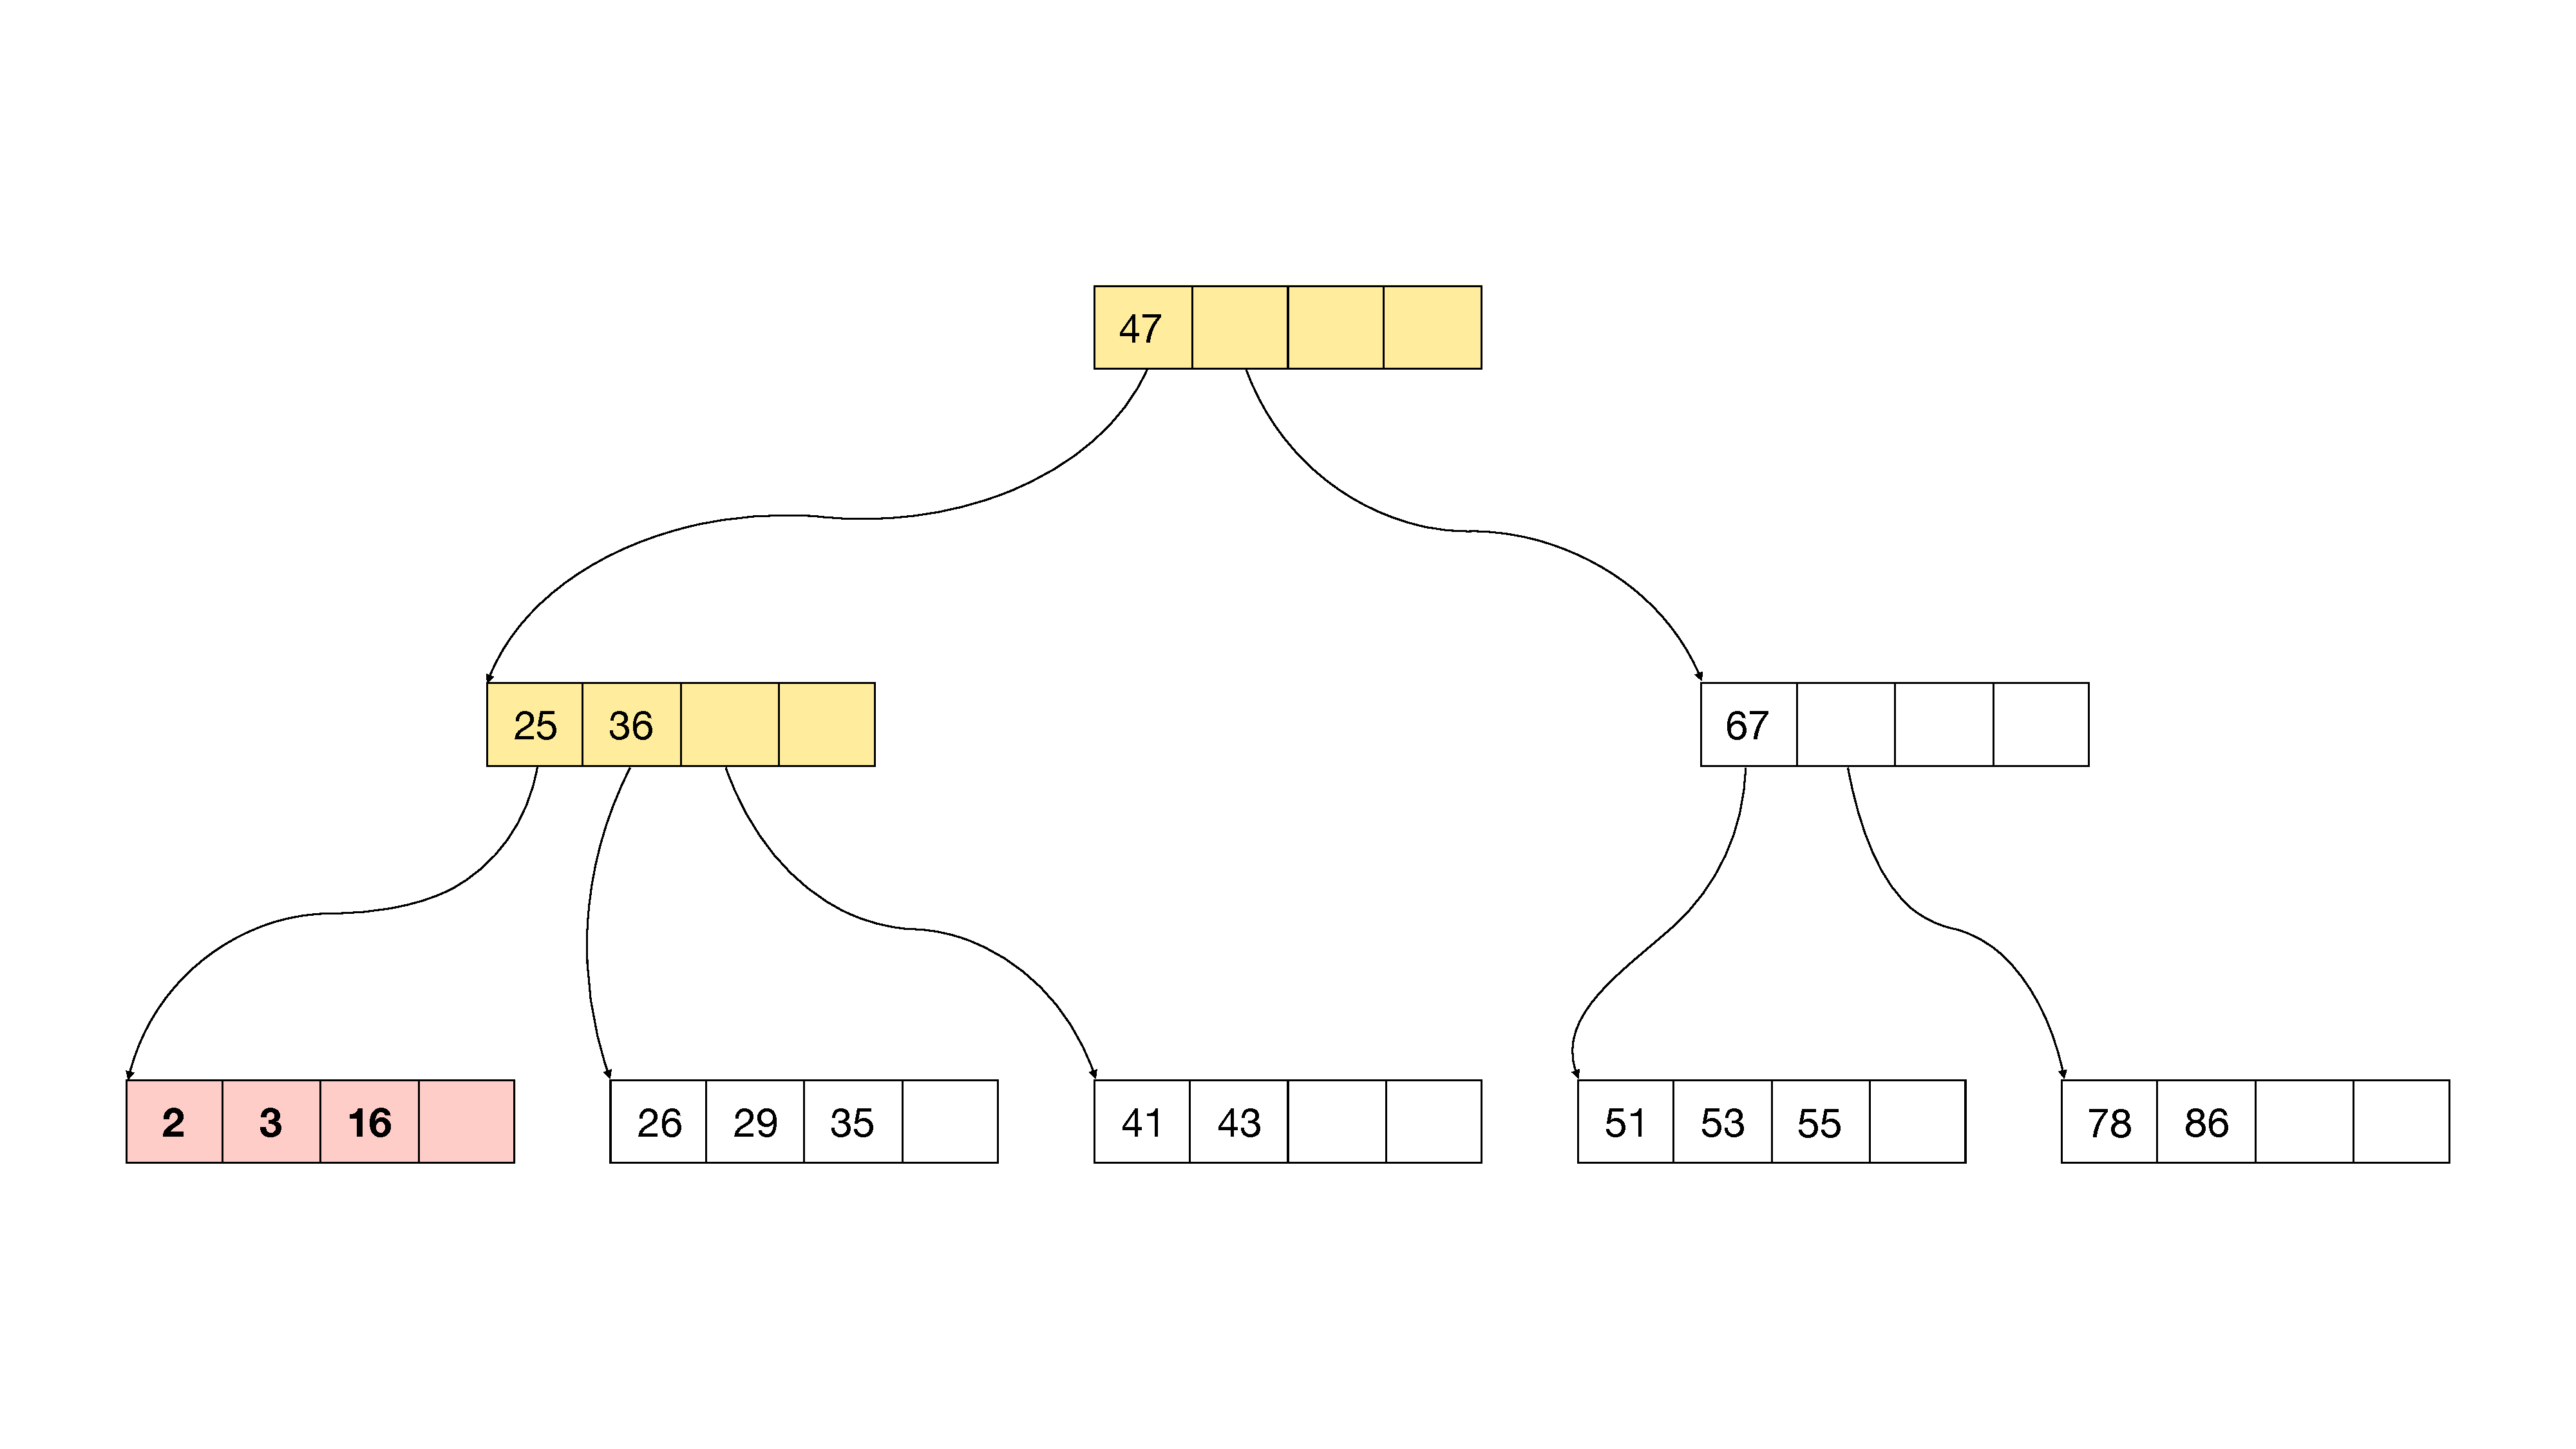
\includegraphics[width=\textwidth]{figures/sequential_access.pdf}
    \caption{Sequential Access Pattern: Updating keys \{2, 3, 16\}.}
    \label{fig:second-pdf}
  \end{subfigure}
  \hfill
  \begin{subfigure}[t]{0.95\textwidth}
    \centering
    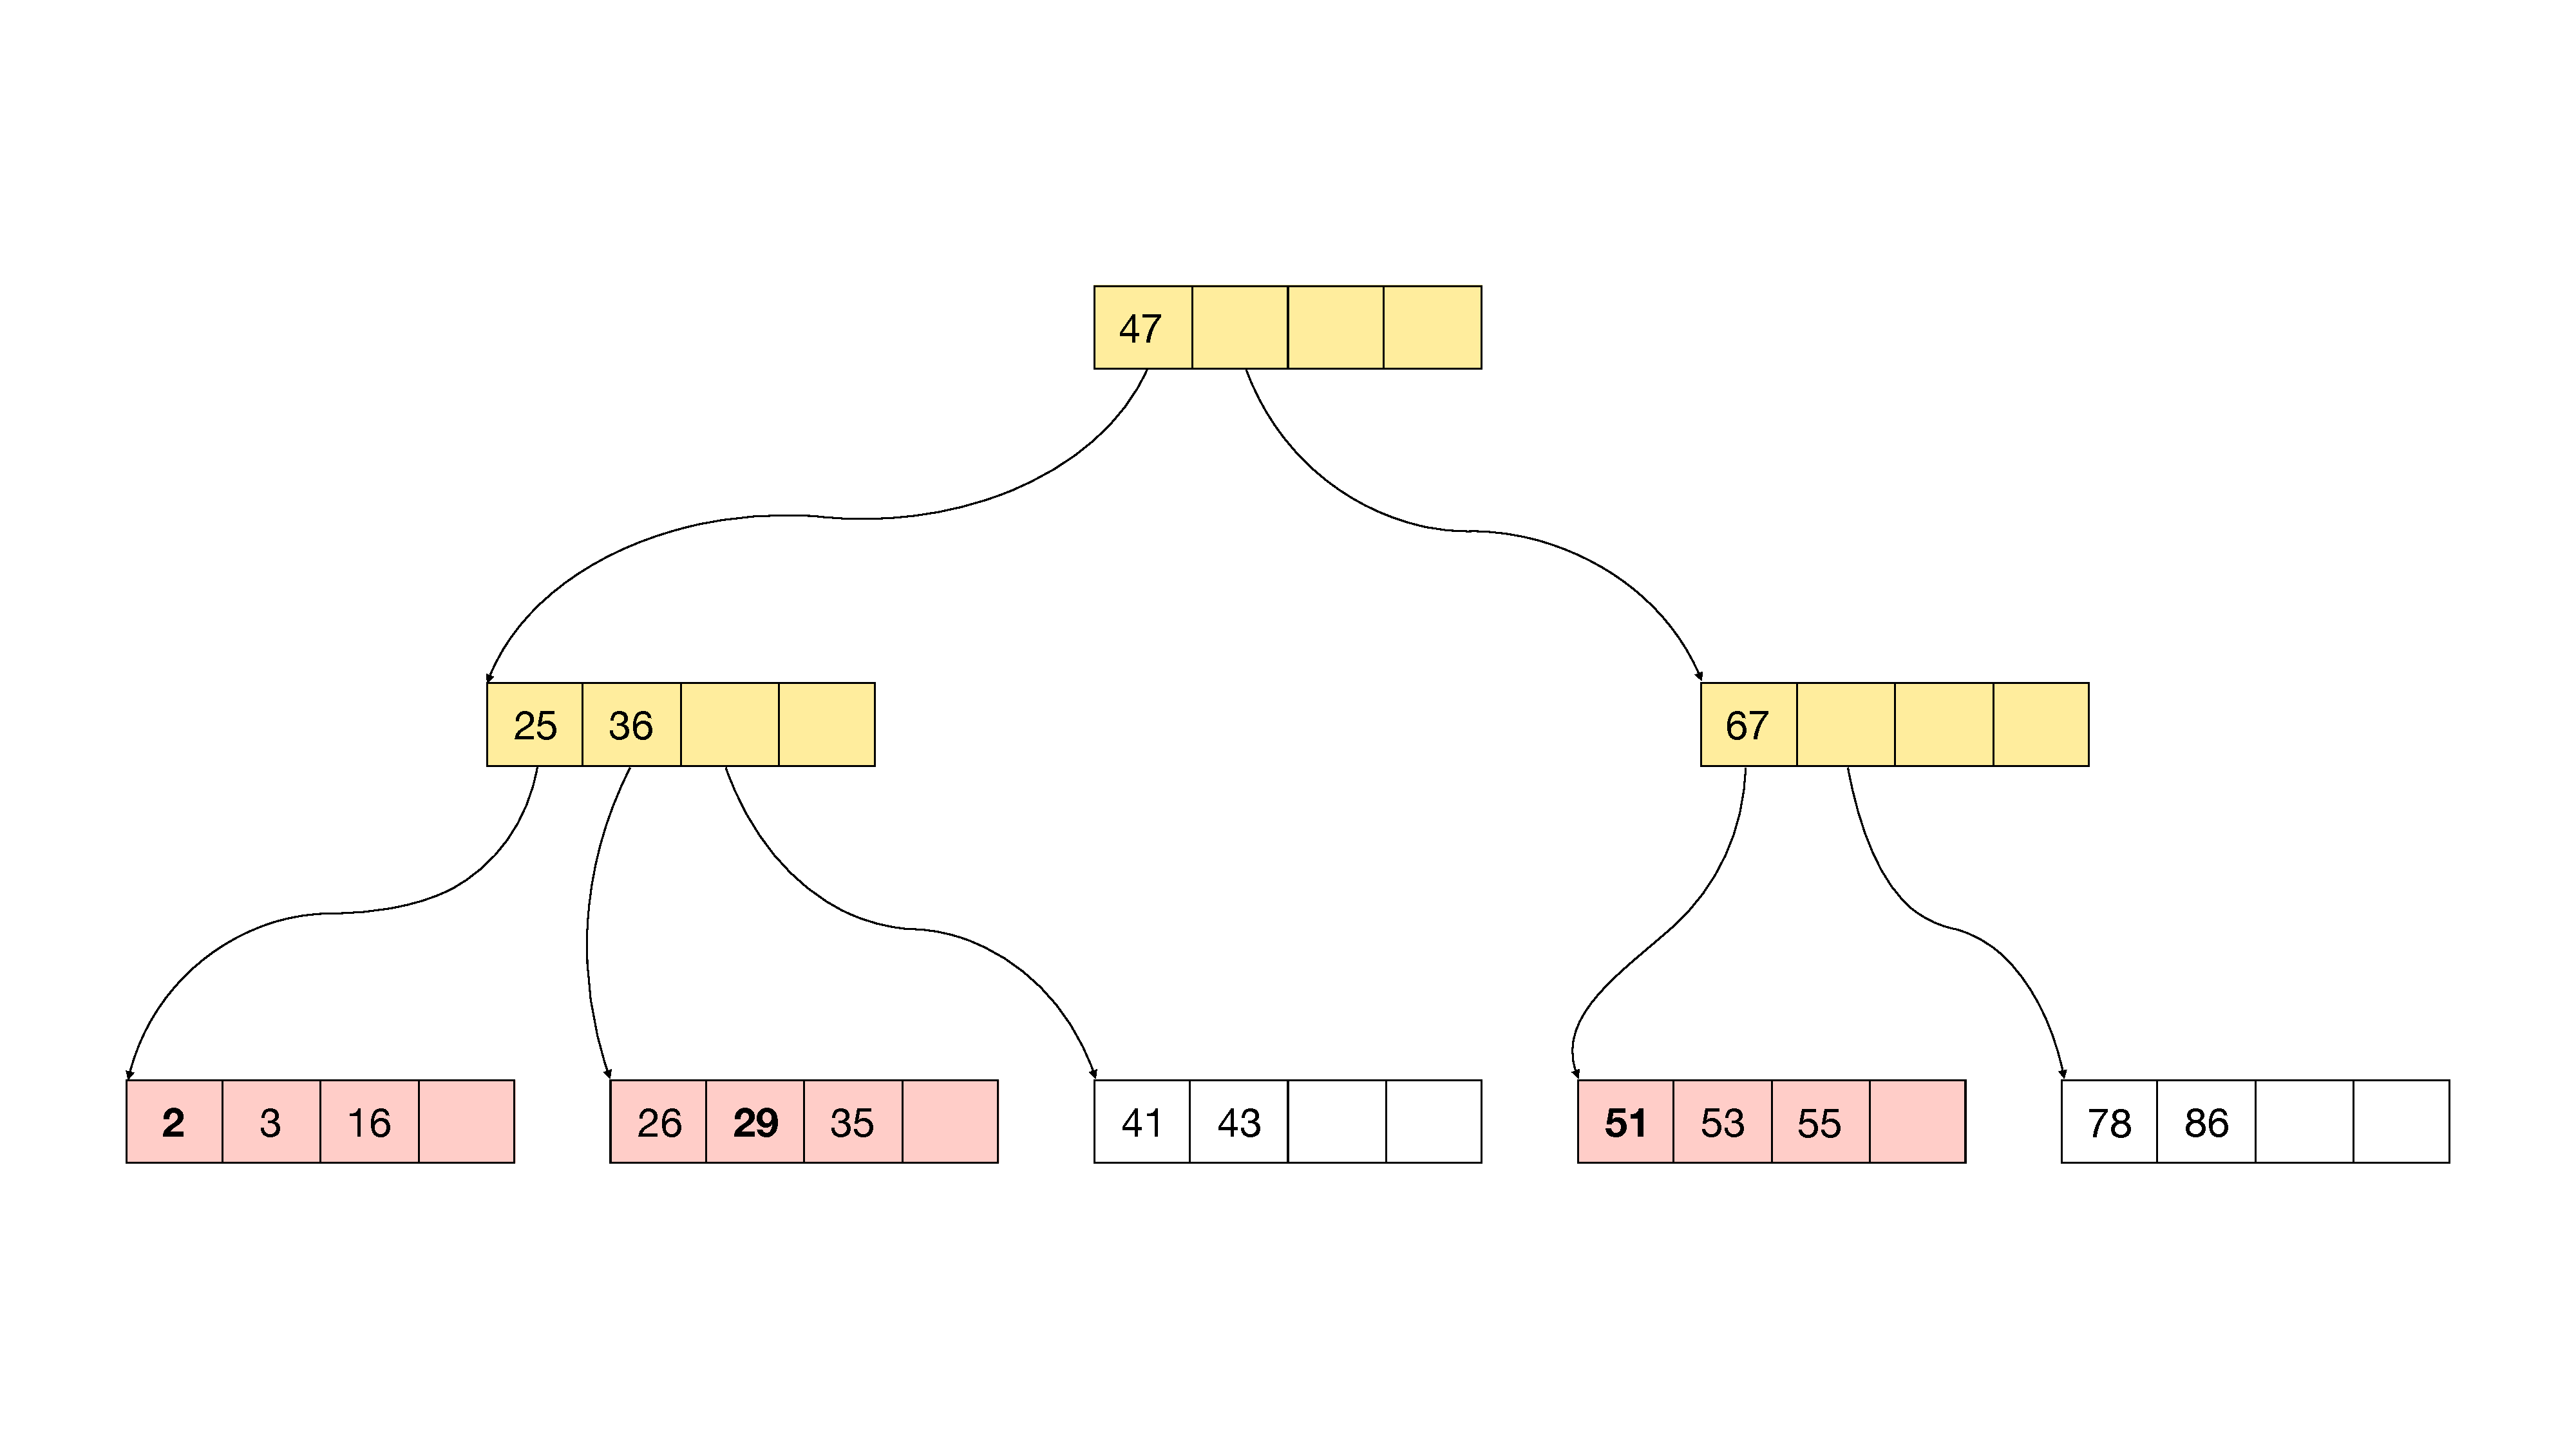
\includegraphics[width=\textwidth]{figures/random_access.pdf}
    \caption{Random Access Pattern: Updating keys \{29, 51, 2\}.}
    \label{fig:first-pdf}
  \end{subfigure}
  \caption{Comparison of access patterns in a B-tree. Written pages are highlighted in red. Read pages are highlighted in yellow.}
  \label{fig:access-pattern-comparison}
\end{figure}

Efficiently managing large data sets is a core requirement for database systems. 
% Not only have \ac{SSD} become drastically cheaper, they also achieve excellent throughput, making them an attactive, cost-effective storage medium \cite{haas2023modern}.
% Yet, external storage accesses remain magnitudes slower than main memory accesses.
% The largest overhead in beyond memory systems lies in \ac{IO} operations on external storage. 
Therefore, minimizing \ac{IO} operations remains the fundamental premise for designing modern, high-performance \ac{DBMS}.
Primarily, this is done by caching frequently accessed pages in \ac{DRAM} using a buffer manager \cite{leis2018leanstore}.
The system stores data in pages, which the buffer manager can cache and uniformly serve to all components in the system.
This modular design separates concerns between the buffer manager and its users, such as indexes and data structures.
However, this also means that the buffer manager is agnostic of user access patterns.
While the buffer manager minimizes the number of \ac{IO} operations, to the best of its knowledge, every system component must design its access patterns to be as efficient as possible. 

A prominent example of such a component is the B-tree \cite{bayer1970organization}.
B-trees are the dominant data structure for indexing large datasets in disk-based \ac{DBMS} due to their excellent lookup performance, support for range queries, and simplicity.
However, random writes, a prevalent pattern for secondary indexes, lead to inefficient access patterns that a buffer manager cannot hide for out-of-memory workloads.

B-trees organize their nodes as pages. 
Due to their sorted order, accessing random keys leads to random accesses of different pages, which the buffer manager must load into the buffer.
At eviction time, each modified page requires a complete rewrite to storage, even if only a small portion of the page has changed.
\autoref{fig:access-pattern-comparison} illustrates this effect by comparing a B-tree's sequential and random update patterns.
We consider three updates to the tree.
In the sequential update, the B-tree reads only three pages and writes to one of them.
In the random update, the B-tree reads six pages and writes to three of them.
Merely changing the access pattern from sequential to random leads to a threefold increase in the amount of data written to storage.
Assuming that each page is 4 KB, the sequential update requires one storage write of 4 KB.
The random update requires three storage writes of 12 KB in total.
Random writes introduce \emph{write amplification}, a phenomenon where the amount of data written to storage is significantly larger than the amount of data that logically changed.

Write amplification inflates \ac{IO} operations, wastes bandwidth, and ultimately increases latency in bandwidth-bound scenarios.
For example, in cloud environments, where storage can be remote, an unnecessary network round-trip directly translates to increased latency and reduced throughput in the system.

Additionally, the \ac{SSD} has its own internal write amplification due to its flash translation layer performing garbage collection \cite{haas2023modern}. 
This leads to a multiplication of unnecessary physical writes, wearing out the device faster.

In summary, to design a truly efficient, high-performance system, we must minimize \ac{IO} operations in all components of the storage stack. 
This thesis focuses on closing the efficiency gap in B-trees by reducing write amplification.

\section{Problem Statement}
% Include metrics for write amplification. Why B-trees suffer from it. State the gap.
While B-trees are the backbone of indexing in modern storage engines, their in-place updates introduce significant write amplification, leading to performance degradation and reduced device lifespan. 

\ac{LSMT} address write costs by always writing sequentially, but they introduce high read amplification and complex tuning requirements, making them unsuitable for general-purpose database systems.

B$\epsilon$-Trees buffer and batch updates starting from the root and propagating them down the tree to reduce write amplification. 
Firstly, this introduces two searches per node, one for the next pivot and one for a buffered update for the looked-up key.
Secondly, the reduced space for pivots in each node reduces the fanout of the tree, leading to taller trees and more \ac{IO} operations per lookup.
Most importantly, though, it significantly limits concurrency in the data structure, as the hottest nodes are locked for more extended periods of time to write the update messages, reducing throughput in the tree.

We identify a research gap for a B-tree variant that effectively reduces write amplification while preserving the excellent query efficiency and concurrency traits of traditional B-trees.

% Figure: Show write amplification gap between sequential and random writes. Show difference in latency of inserting x keys, difference in IO operations, difference in written volume.

% Circumvent more robust access patterns using LSM Trees. Sacrifice read performance.
\section{Objectives}
% Explicitly list what your thesis adds to the field.
The primary objective of this thesis is to design, implement, and evaluate a B-tree variant that reduces write amplification while maintaining the high read performance and concurrency of traditional B-trees.
We focus on the following research questions:
\begin{enumerate}
  \item How can we effectively reduce write amplification in B-trees?
  \item How can we preserve read performance and concurrency in the presence of write optimizations?
  \item How does the proposed approach compare to existing methods regarding write amplification, query performance, and throughput?
  \end{enumerate}

While we reflect on significant hardware trends in this thesis, such as the increasing prevalence of \ac{SSD}, we do not target optimizations for specific hardware features.
Instead, we aim to design a solution that is broadly applicable across different storage media and hardware configurations.

We also do not aim to outperform \ac{LSMT} in write-intensive workloads, as they are fundamentally optimized for such scenarios, trading off lookup performance.

While the page-oriented design is one reason for \ac{IO} amplification in B-trees in general, we do not aim to redesign the data structure from the ground up.
Instead, we focus on a lightweight extension to the traditional B-tree that can be integrated into existing systems with minimal changes.

\section{Contributions}
% Summarize the main contributions of your thesis.
This thesis introduces 3B-tree, a B-tree variant incorporating a lightweight buffering layer to minimize write amplification.
The buffering layer batches small write operations, reducing the frequency and volume of writes to external storage.
% Instead of changing the B-tree structure itself, we introduce a secondary data structure, the Delta Tree, that buffers changes to B-tree nodes.
When the buffer manager evicts a B-tree node from memory, we determine whether it has changed significantly enough to warrant a full write to storage.
If not, we buffer the changes.
% When loading a B-tree node from storage, we apply any buffered changes from the Delta Tree to reconstruct the most recent state of the node.
Essentially, we minimize \ac{IO} operations to those strictly necessary. 

The novelty of our approach lies in its non-intrusive design: 
We only perform additional operations when the buffer manager exchanges B-tree nodes between memory and external storage.
In contrast to other approaches (see \autoref{chap:related-work}), we neither alter the B-tree structure its fundamental operations, nor impact concurrency in the tree.
We keep read amplification low by only introducing additional lookups during page reads.
Our approach is easy to integrate into existing systems and preserves the desirable properties of traditional B-trees.

We hereby contribute to the broader effort of minimizing the overhead of beyond memory systems and designing efficient, high-performance database systems for modern hardware.

\chapter{Background}
This chapter provides the necessary background for understanding the problem of write amplification in B-trees and the proposed method by outlining the characteristics of external storage, the architecture of database systems, and the behavior of B-trees in out-of-memory environments. 
Furthermore, it introduces the concepts of write, read, and space amplification, which allow for a differentiated analysis of index structures for their efficiency and performance characteristics.

\section{External Storage Characteristics}
For some time, in-memory database systems like Hyper \cite{kemper2011hyper} have gained popularity due to the decreasing cost of \ac{DRAM}.
However, that trend has reversed recently, as \ac{DRAM} prices have stagnated \cite{haas2023modern} and \ac{SSD} price-performance-ratios have improved significantly \cite{leis2024leanstore}.
Therefore, modern database systems are designed to operate efficiently on external storage and since index structures are the performance-critical component, out-of-memory indexing has become a key consideration again.
B-trees have been the dominant index structure for out-of-memory indexing, since their high fanout minimizes the number of \ac{IO} operations.

Historically, hard disks were the dominant storage medium.
Hard disks have a significant imbalance in latency between random and sequential \ac{IO} due to their mechanical nature.
While \ac{SSD} have a smaller difference between random and sequential \ac{IO}, they still exhibit asymmetric performance, especially in writes \cite{haas2023modern}.
Therefore, to amortize the cost of random \ac{IO}, database systems and their index structures are designed to access data in pages of multiple kilobytes instead of individual tuples.
This assumes that subsequent accesses exhibit some locality, which is often the case in practice.
While we will be referencing disk-based systems throughout this thesis, we speak of systems operating on external storage, which can be either disk-based or flash-based.

\section{Database System Architecture Overview}

% TODO: Mention that we don't consider writes to the log which should be the same in all systems.
% TODO: Work in equations and read/space ampl. from "A Comparison of Fractal Trees to Log-Structured Merge (LSM) Trees" https://www.cs.cmu.edu/~dga/papers/sigmod10-fractal.pdf

\begin{figure}[htpb]
  \centering
  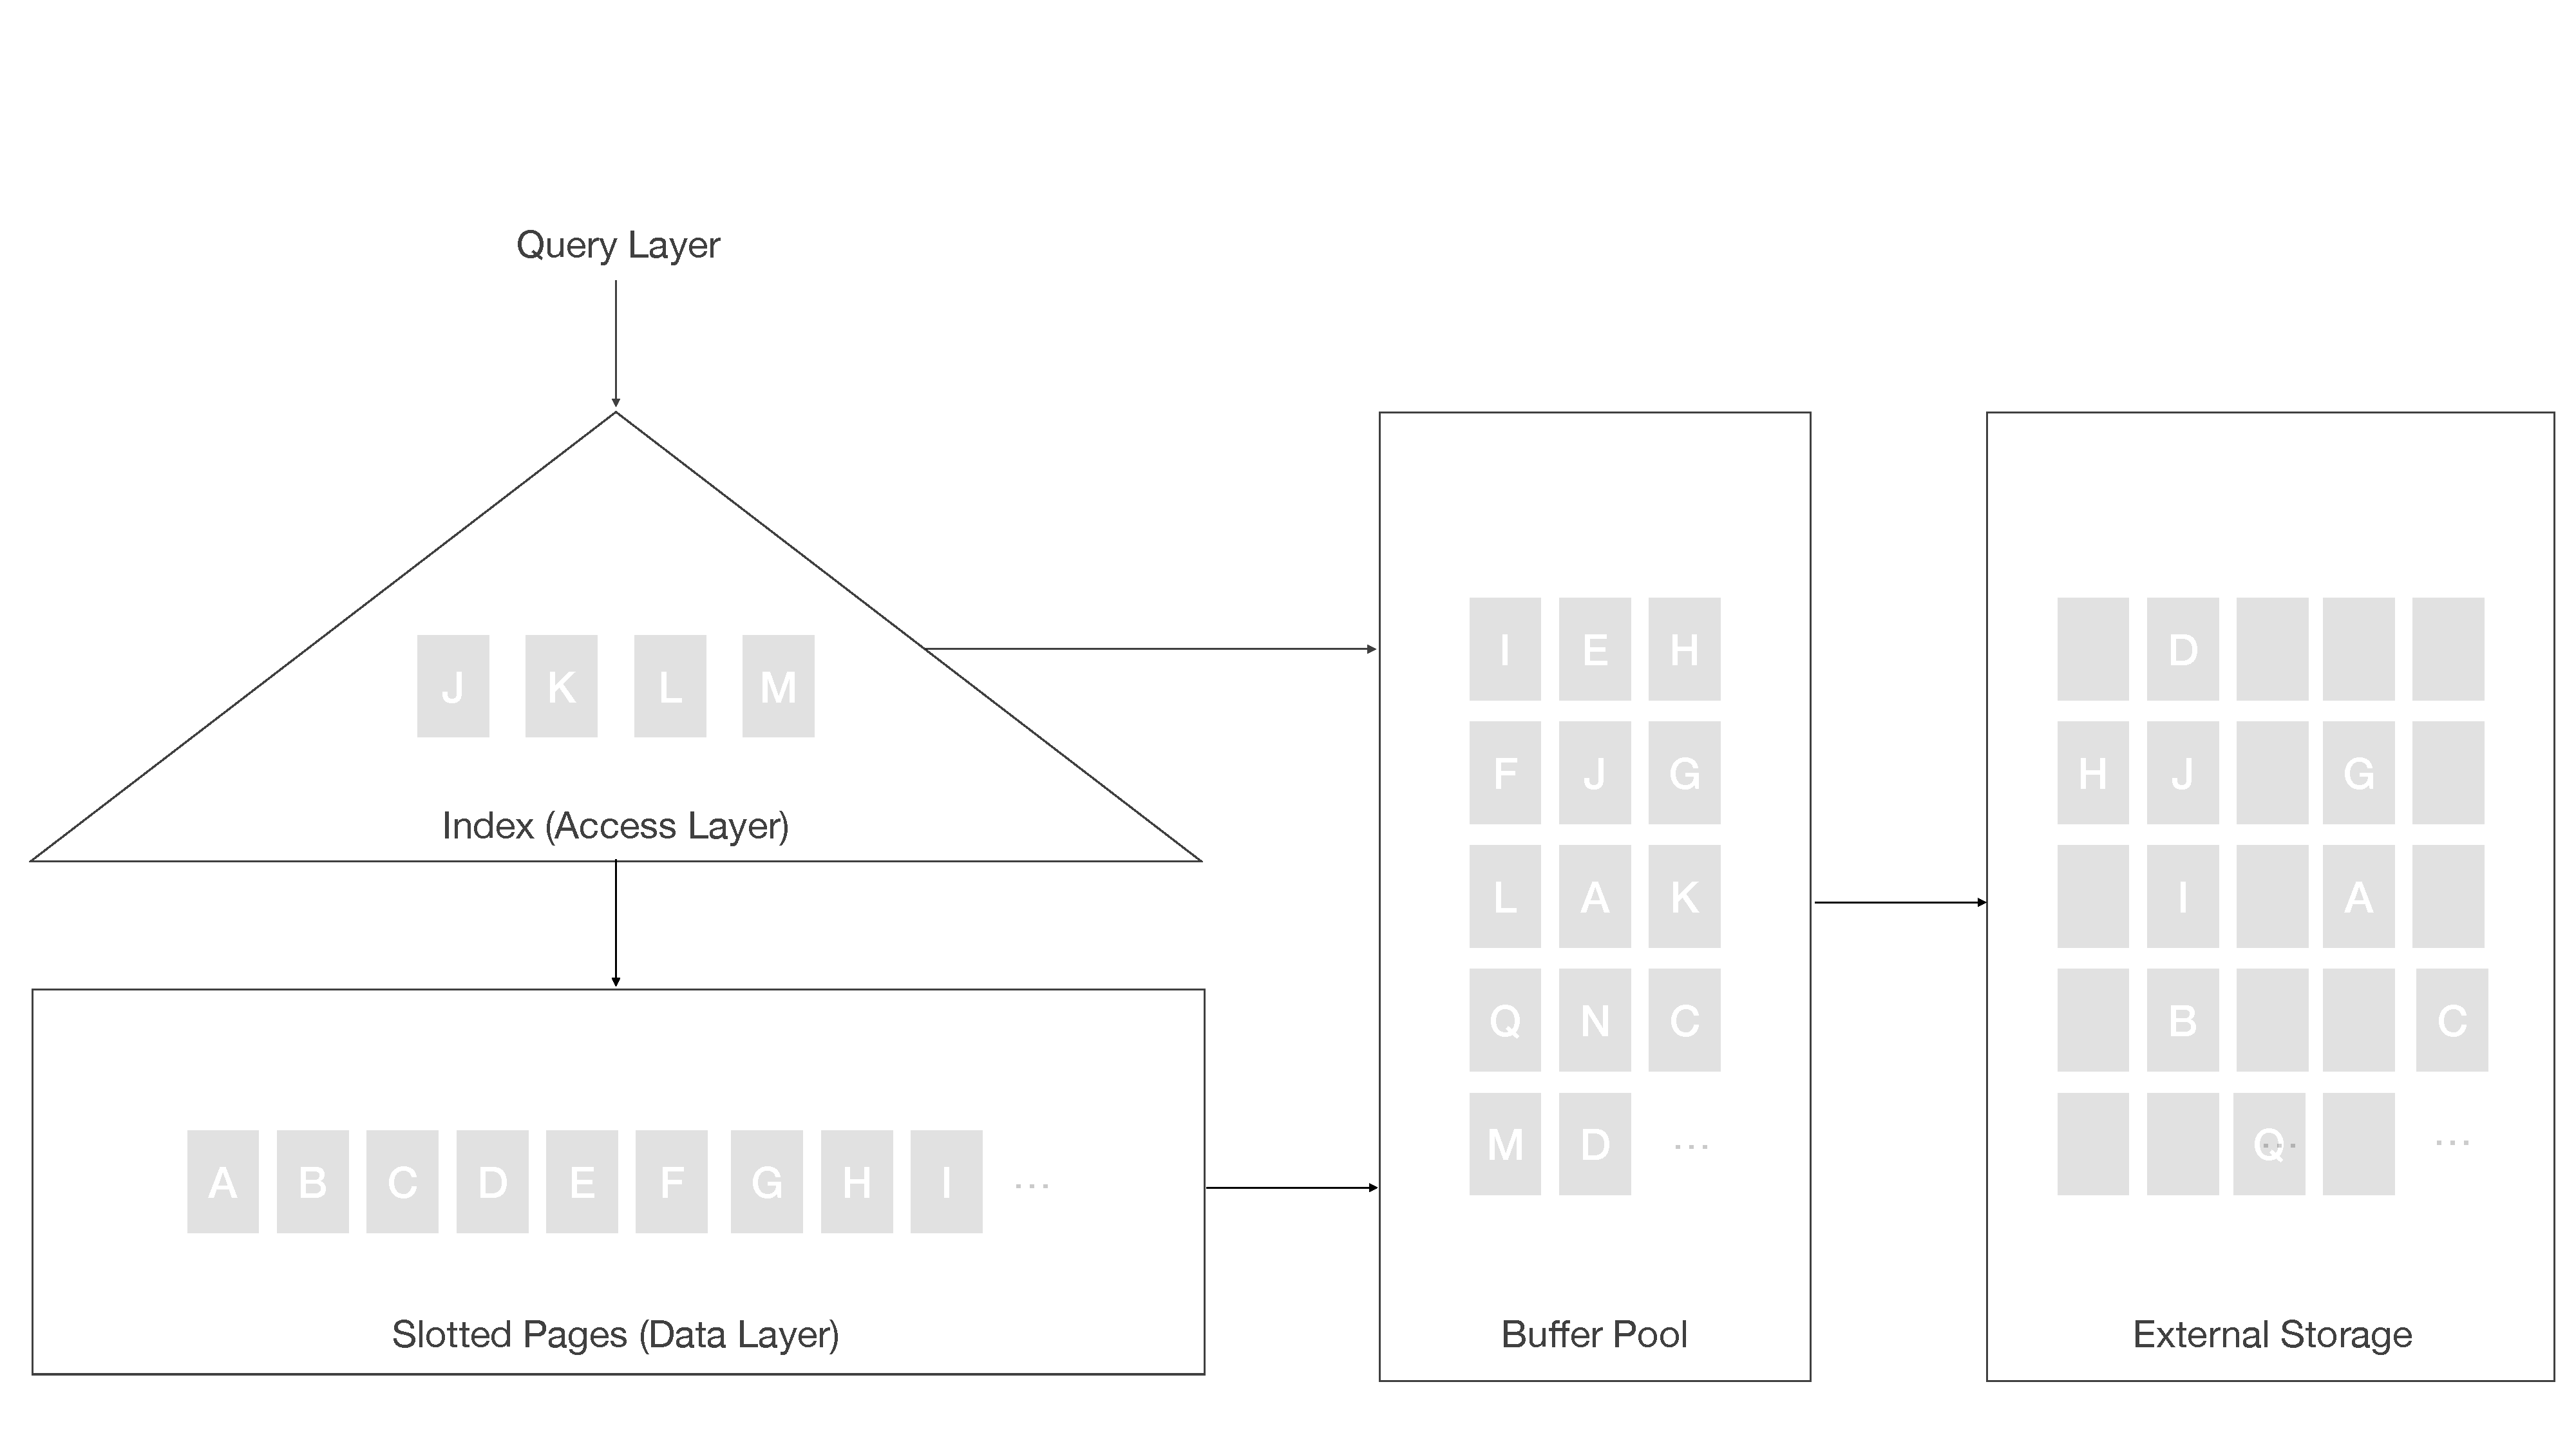
\includegraphics[width=0.99\textwidth]{figures/db_architecture.pdf}
  \caption{The storage and access layer of a database system. The index provides access to the tuples stored in the slotted pages. Each component requests data from the buffer manager, which handles caching and loading pages from external storage. Adapted from "Database Systems on Modern CPU Architectures" \cite{mdbs2024slides}.}
  \label{fig:db-architecture}
\end{figure}

In the scope of this thesis we focus on a classic architecture of a single-node, disk-based database system.
Note that this architecture is not a constraint of our method, which can be applied to any database system using B-trees as an index structure.
However, for clarity, we describe our method in the context of this architecture.

The access and storage layer of a database system typically consist of a buffer manager, one or more index structures and the slotted pages that store tuples identified by \ac{TID}s, as illustrated in \autoref{fig:db-architecture}.
Since we operate in a beyond memory setting, the buffer manager is responsible for caching pages in \ac{DRAM} and loading them from external storage when needed.
Therefore, all components accessing physical data interact with the buffer manager to load and store their pages.
When a query is executed, the index is accessed by a given key (e.g. the primary key) to find the \ac{TID} of the relevant tuple.
The index is typically stored in pages, which are loaded into the buffer pool by the buffer manager.
Using the \ac{TID}, the corresponding tuple can be retrieved from the slotted pages.
The \ac{TID} encodes the \ac{PID} and the slot number within the page.
When a tuple is updated, the corresponding page is loaded into the buffer pool, modified, and marked as dirty.
Should the buffer pool be full, the buffer manager evicts pages based on its replacement policy.
Clean, unchanged pages can be discarded, while dirty, modified pages must be written back to external storage.

\section{Index Structures}
Index structures are data structures that enable efficient access to data stored in a database.
Typically, they map a key to a constant, unique \ac{TID}.
Ideally, the \ac{TID} nevers changes, as this would require all indexes pointing to that tuple to be updated.
Keys can be arbitrary types and therefore of fixed or variable size, such as integers or strings.
We will consider both within this thesis.
When the key of a tuple changes, the index must be updated to reflect the new key.

Some key-value stores directly map keys to tuples within their index structure, omitting the indirection via \ac{TID} and slotted pages.
However, in a general purpose \ac{DBMS}, we typically want to support multiple indexes on the same data.
If we stored tuples directly in the index, we would need to update all indexes when a tuple changes.
Therefore the access and storage layer are decoupled via \ac{TID}s.
For the context of this thesis, however, it does not matter whether the index maps keys to \ac{TID}s or directly to tuples.

Indexes can be classified into primary and secondary indexes.
A primary index is built on the primary key of a table, which uniquely identifies each tuple.
A secondary index is built on a non-primary key, which can be non-unique.

Consider the following example use-case: a user database with a primary key on the user ID and a secondary index on the email address.
When inserting several new users, we update the indices.
The primary index is updated with an auto-incrementing user ID, thus, the primary key follows a sequential access pattern.
However, the email addresses of new users are likely to be random and not follow any specific order.
Therefore, if the secondary index is sorted on the keys, as they are in a B-tree, the index exhibits a random access pattern.
Such access patterns have implications on the performance of index structures, as we will discuss in the following sections.

% TODO: SSD Wear Leveling? Garbage Collection? Wearout? https://www.vldb.org/pvldb/vol18/p4295-haas.pdf

\section{B-trees}

\begin{figure}[htpb]
  \centering
  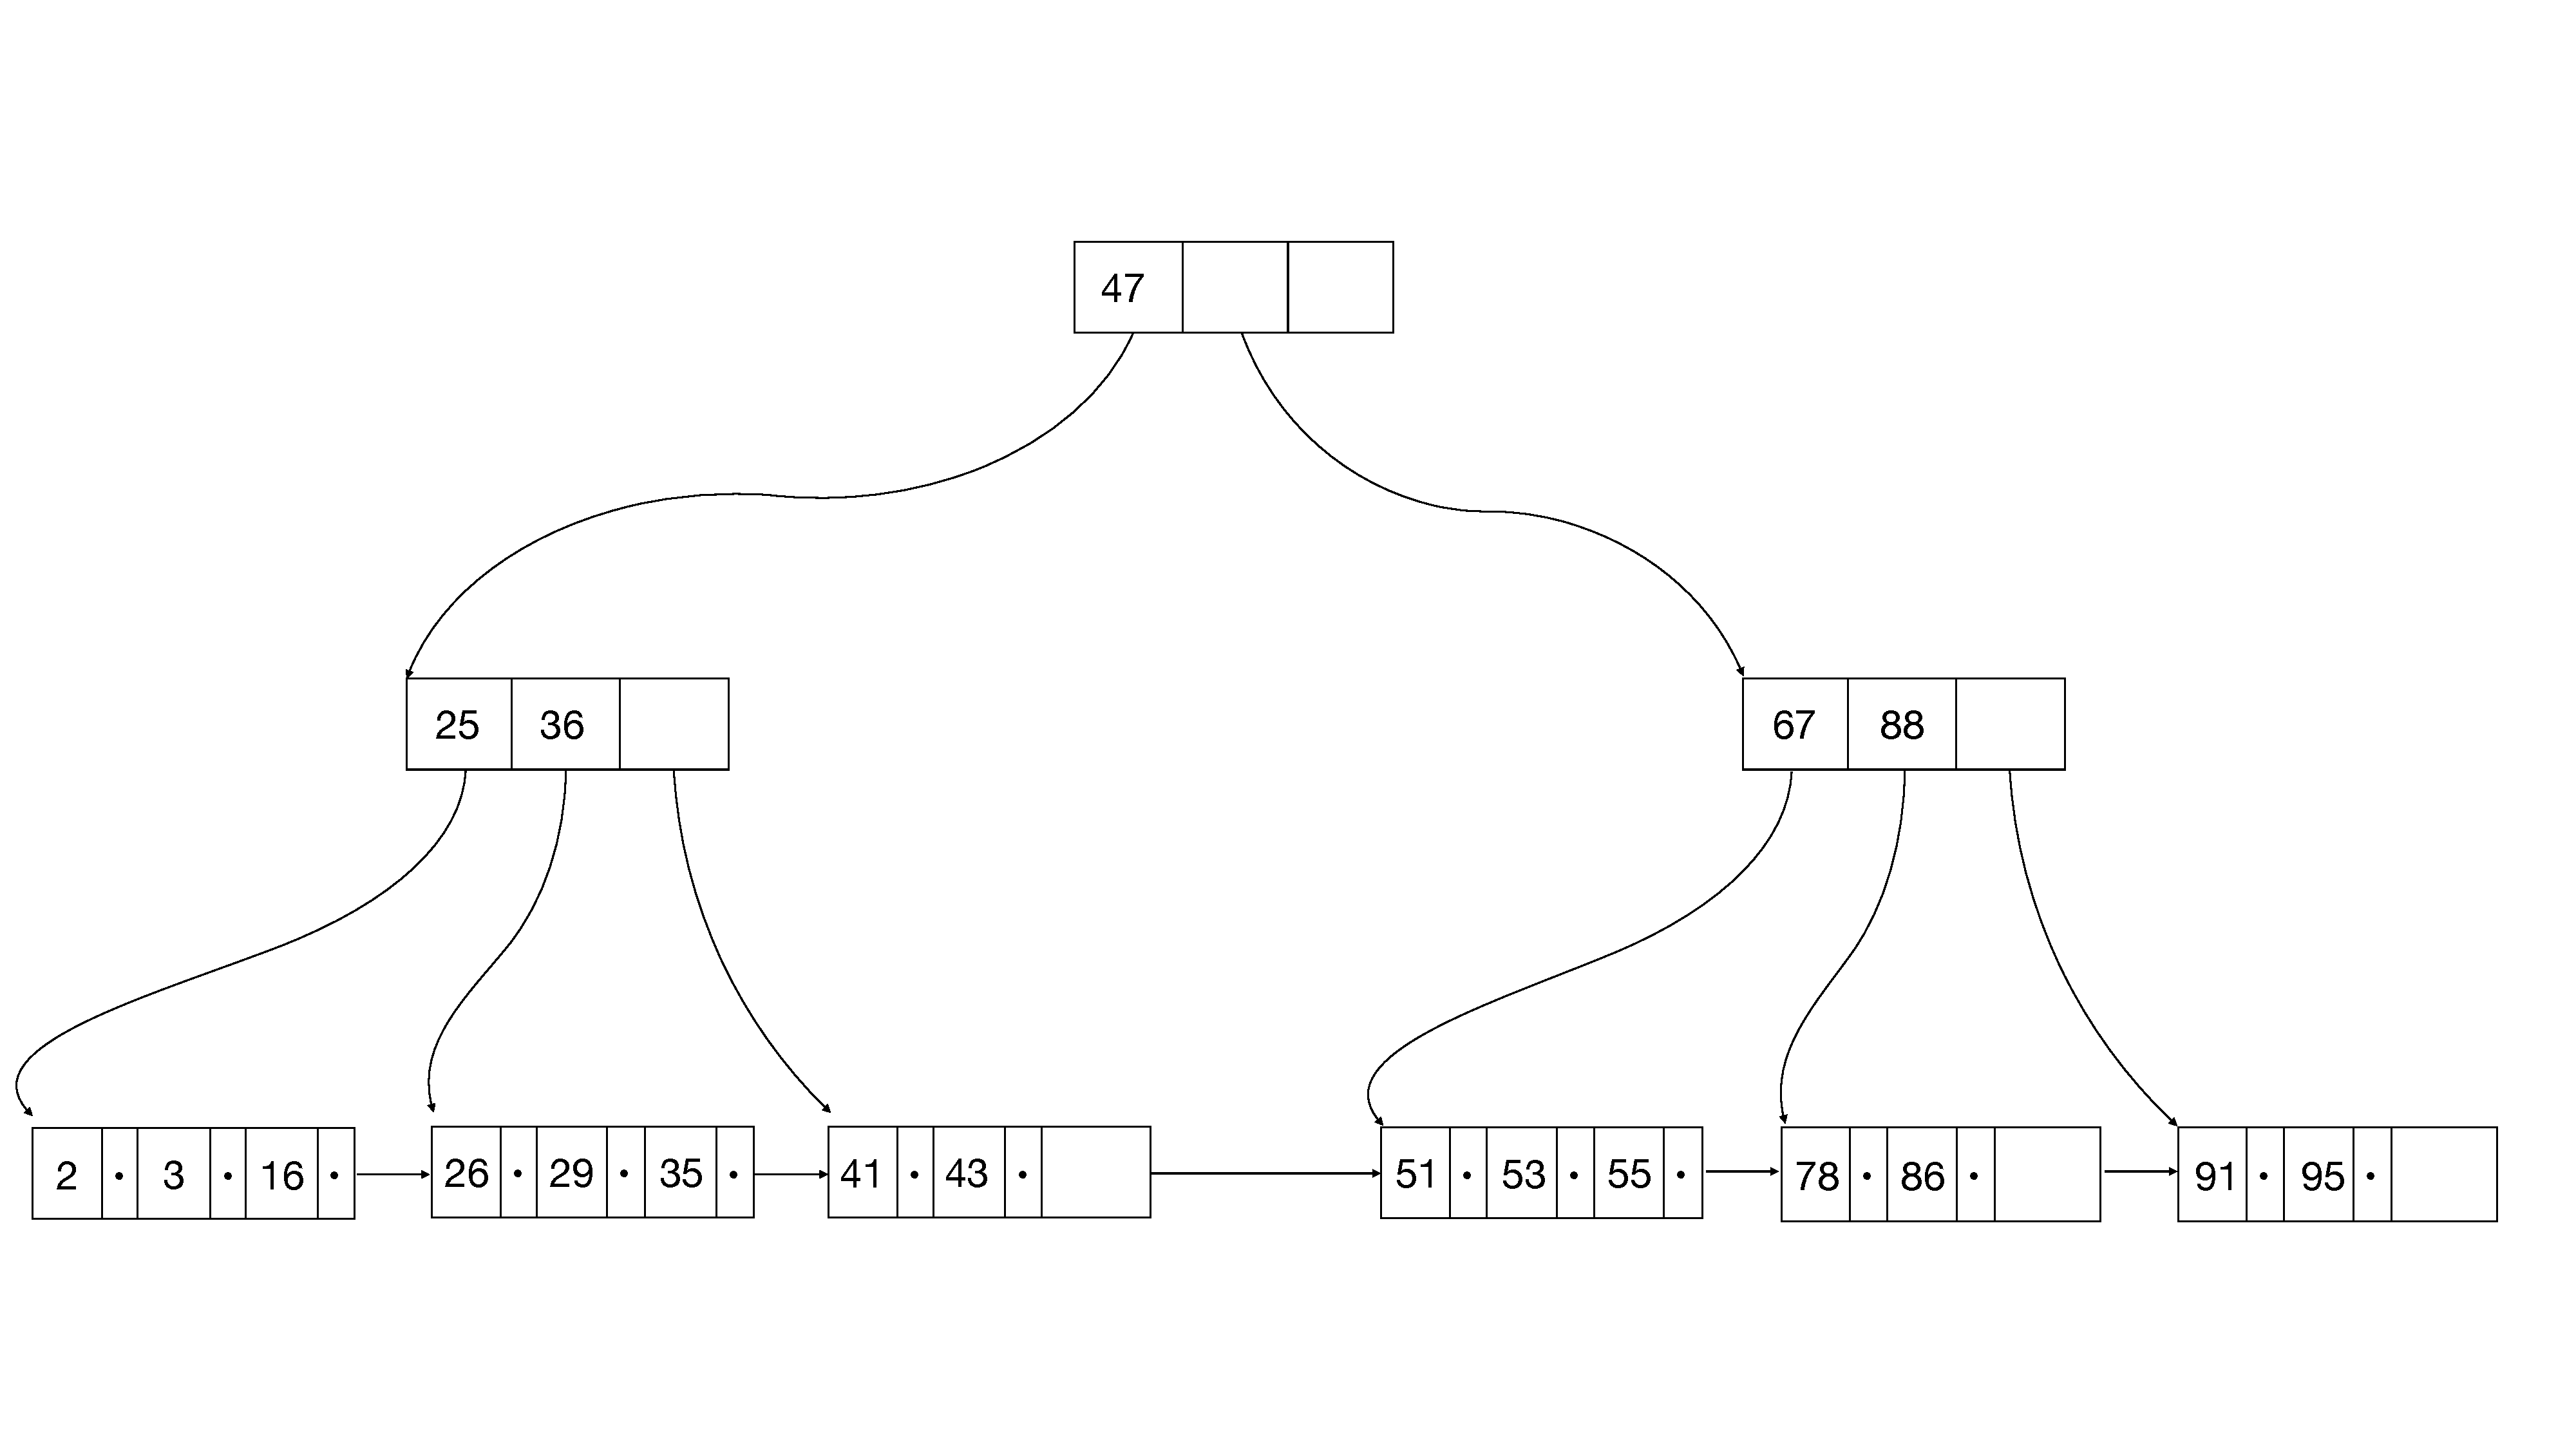
\includegraphics[width=0.99\textwidth]{figures/b_tree.pdf}
  \caption{A B+-tree. Child pointers are represented as arrows. Values (the \ac{TID}) are represented as bullet points •.}
  \label{fig:B-tree}
\end{figure}

B-trees \cite{bayer1970organization} are a self-balancing tree data structure that maintains sorted data and allows for insertion, deletion, and search operations in logarithmic time, $\mathcal{O}(\log n)$, where $n$ is the number of entries in the tree.
A B-tree is organized in fixed-size pages, called nodes. These pages are transferred and cached transparently by the buffer manager between external storage and \ac{DRAM}.
Each node can split off a sibling once it is full. If a node is full and a new key needs to be inserted, the node splits into two nodes, and the middle key is promoted to the parent node.
Additionally, nodes can merge with a sibling if they become less than half full. For simpliticity, we omit merging of nodes in this thesis.

The tree only increases in height when the root node splits.
Each node contains between 2 and 2k entries, except for the root node, which can contain between 1 and 2k entries.
Each entry is a triple of a key, a pointer to a child node, and optionally a value (the \ac{TID}).
The entries in each node are sorted by key. On leaf nodes (nodes without children), the pointer to a child node is undefined.
An inner node (a node that is not a leaf) with k keys has k+1 children.
Each entry in an innder node separates the key space of its children.
The additional child pointer is necessary to separate the key space above the largest key in the node.
For example, consider an inner node with keys \{10, 20, 30\}.
The first child contains all keys less than 10, the second child contains all keys between 10 and 20, and the third child contains all keys between 20 and 30. 
The fourth child contains all keys greater than 30.

When searching for a key in the tree, we start at the root node.
On each node, we perform a binary search to find the appropriate pivot key and follow the corresponding child pointer.
We stop when we reach a node with the desired key.

\subsection*{B+-trees}
When addressing B-trees in this thesis, we actually refer to B+-trees, a variant of B-trees where all values are stored in the leaf nodes and internal nodes only store keys and child pointers to guide the search.
The separator keys in internal nodes may or may not occur in the data. An example B+-tree is illustrated in \autoref{fig:B-tree}.
The lookup procedure is the same as in a B-tree, however we always traverse the full tree from root to leaf to find a key.
Not only does this simplify the B-tree logic, it also increases the fanout of inner nodes, leading to a lower tree height and therefore fewer \ac{IO} operations for lookups since less pages are involved in reaching the leaf level.
Also, it allows for efficient range queries by scanning the leaf nodes in order.
Due to its excellent lookup performance, support for range queries, and simplicity, B+-trees are the dominant data structure for external storage \cite{mdbs2024slides}.

% TODO: Cut this subsection?
\subsection*{Disk-Access-Model}
To analyze the performance of B-trees in a beyond memory setting, we use the \ac{DAM} \cite{aggarwal1988complexity} \cite{kuszmaul2014fractal}.
The model has two levels of memory: an internal memory of size $M$ and external storage of infinite size.
The storage device is organized in fixed-size pages, which are the units of data transfer between memory and storage and determine the size of nodes in a B-tree.
For simplicity of this analysis of the \ac{DAM} for B-trees, we assume that records are constant sized (An assumption that simplifies this explanation but does not hold in practice. 
Therefore we will \textbf{not} assume this in our method and implementation.) and that nodes are always completely filled.
When a database has $N$ records, and the storage device has pages of size $P$, the B-tree has a height of $\log_P(N/P)$, where inner nodes contain $O(P)$ children and leaf nodes contain $O(P)$ records.

Each lookup/insertion/deletion requires a traversal from the root to a leaf node, leading to $\mathcal{O}(\log_P(N/P))$ \ac{IO} operations.
Since the majority of nodes in the tree are leaf nodes, we can assume that most inner nodes can be cached by the buffer manager.
In that case, we would require only a single \ac{IO} per B-tree operation.

In practice, B-trees are often used to index variable-sized keys and values.
Therefore, we will consider variable-sized records in our method and implementation.
However, the \ac{DAM} provides an approximation.

% TODO: Slotted Node Layout here or in Implementation?

\subsection*{Node Size \& Fanout}
\label{sec:node-size-fanout}
The node size (i.e. the page size) is a crucial parameter in the design of a B-tree, as it affects the height of the tree.
Larger nodes lead to more entries per node, increasing the fanout for inner nodes and decreasing the height of the tree.
When we can address more children per node, we need fewer levels in the tree to address the same number of keys.
Since every lookup/insert/delete operation requires a traversal from the root to a leaf node, fewer levels lead to fewer pages involved in the lookup.
Thus, larger nodes lead to fewer \ac{IO} operations per lookup.
Additionally, since we need fewer distinct pages, we induce less page management overhead in the buffer manager.

Large nodes are particularly beneficial for analytical, read-heavy workloads, which often perform large scans and are interested in large parts of the data.
However, workloads that perform many updates and point queries, are sometimes only interested in a small portion of the page.
As a result, larger nodes lead to more \ac{IO} amplification, as we read and write significantly more data than necessary to perform the operation.
If subsequent operations follow a sequential access pattern, the \ac{IO} amplification is not a problem, as we will be operating on pages already cached by the buffer manager.
Ideally, no or very few additional \ac{IO} operations are necessary.
With random access patterns, however, this \ac{IO} amplification due to large page sizes becomes a problem.
% Modern \ac{SSD} were shown to perform best at page sizes of 4 KB \cite{haas2023modern}.

% TODO: Make sure this is still correct by the end of the thesis:
While we will be evaluating performance under different node sizes, this tuning parameter is not the primary focus of this thesis.
Instead, we focus on reducing \ac{IO} amplification in B-trees at any page size.
However, larger nodes are expected to profit more significantly from our approach, as they induce more \ac{IO} amplification in B-trees.


\section{Write Amplification}
Write amplification is the ratio of the amount of data written to storage versus the amount of logical data written by the user.
For example, if the database updates an entry of 64 B, but needs to write a full page of 4 KB to storage, the write amplification is 4096 B / 64 B = 64.
Write amplification $WA$ is formally defined as:

\[
WA = \frac{Bytes Written Physically}{Bytes Written Logically}
\]

There are multiple layers of write amplification in a database system, which we need to differentiate from each other.

\inlinesection{Application Layer.}
At the application layer, we consider an external end user interacting with the database system, e.g. through SQL.
When an end user inserts a tuple through a query, the database system must insert the tuple in the table itself, in the \ac{WAL} and all indexes that serve to access the tuple later.
Consequently, we write significantly more bytes than the user requested logically.
Additionally, updating a B-tree index might cause structural changes such as node splits or merges that create new nodes, delete new nodes and update the parent nodes.
Thus, a database system inherently comes with write amplification merely to perform its purpose: manage data.
This is not the focus of this thesis; we consider all updates to tables, data structures and the \ac{WAL} as necessary and focus on reducing write amplification within the index layer specifically.

% TODO: We kinda do measure write amplification on this layer as well as bytes inserted not "B-tree" as the user.
\inlinesection{Index Layer.}
At the index layer, we consider the B-tree as the user of pages.
When a B-tree entry is updated, the bytes written logically include not only the updated key but also any additional metadata required to maintain the tree structure.
This can include information about node splits, merges, and the promotion of keys to parent nodes.
The writes are amplified by the B-tree's page structure that requires rewriting the entire page even if only a small portion has changed.
As mentioned in \autoref{sec:node-size-fanout}, the node size directly impacts the write amplification at this level.
This is the write amplification we focus on in this thesis, by minimizing the number of pages written to storage for a given set of updates (see \autoref{chap:method}).

\inlinesection{Physical Layer.}
At the physical layer, we consider the database system as the user (the host) of the physical storage device.
When the database system writes a page to storage, the bytes written logically are the size of the page.
However, due to the characteristics of the storage device, the actual bytes written physically can be larger.
\ac{SSD} typically operate in larger units called blocks, which consist of multiple pages.
When a page is updated, the entire block containing that page must be rewritten, leading to write amplification.
Additionally, when garbage collection is performed, valid pages within a block must be copied to a new block before the old block can be erased and reused.
Recent research observed write amplification factors up to 10x on modern \ac{SSD} \cite{haas2025ssd}.
Consequently, a page write of 4 KB can lead to physical writes of up to 40 KB on the device, using up valuable bandwidth and wearing out the device faster.
While we do not focus on hardware-level write amplification in this thesis, it shows the importance of reducing write amplification at the host level.
Unnecessary writes by the database system are multiplied by \ac{SSD}.

% See Bepsilon paper for more analytical model

% TODO: We kina misuse this term in the evaluation chapter, since we do count the reads, not the total IO upon one read.
\section{Read Amplification}
Read amplification is the number of \ac{IO} operations required to answer a query \cite{kuszmaul2014fractal}.
As described above, a B-tree lookup requires a traversal from the root to a leaf node, which is $\mathcal{O}(\log_P(N/P))$ \ac{IO} operations in the \ac{DAM}, assuming that our cache is cold.
In practice, the buffer manager caches pages in \ac{DRAM}, which can significantly reduce the number of \ac{IO} operations.
To answer range queries, we can scan the leaf nodes in order, which is efficient in B+-trees.
Therefore, we only traverse the tree once to find the start of the range and then scan the leaf nodes sequentially.
Read amplification is a common tradeoff when reducing write amplification, as we will see in alternative data structures (see \autoref{chap:related-work}).
We will analyze the introduced read amplification of our method compared to the traditional B-tree in our evaluation (see \autoref{chap:evaluation}).

\section{Space Amplification}
Space amplification is the ratio of the amount of space used by the data structure versus the amount of logical data stored \cite{kuszmaul2014fractal}.
Most nodes in a B-tree are leaf nodes, which store the actual data.
However, inner nodes only store keys and child pointers to guide the search, inflating the space usage.
Additionally, B-tree nodes are not always completely filled.
Therefore, B-trees exhibit some space amplification.
Space amplification is not the focus of the thesis, however we will analyze space utilization of our method compared to the traditional B-tree in our evaluation (see \autoref{chap:evaluation}).
\chapter{Related Work}
(Position each data structure in their attempt to solve a certain problem and how it does not solve ours yet/well)

\section{Log-Structured-Merge-Trees}

\ac{LSMT} \cite{oneil1996log} are a popular alternative index data structure to B-Trees for write-heavy workloads.
They are increasingly used in key-value stores such as RocksDB at Meta \cite{rocksdb} or BigTable at Google \cite{chang2008bigtable}.

\inlinesection{Basic Structure.}
\ac{LSMT} consist of two main components: an in-memory component and a disk-based component.
The in-memory component is typically implemented as a balanced tree such as a red-black tree, called a MemTable.
The MemTable accepts and applies updates in memory.
Once it is full, it is flushed to disk as a sorted, immutable runs in files called SSTables.
Over time, multiple runs accumulate on disk.
Since those runs may have overlapping key ranges, lookups need to check both memory and multiple disk files to find a key.

To limit the number of runs on disk and improve lookup performance, \ac{LSMT} organize runs into multiple levels, where each level is larger and more data is sorted than in the previous one.
When a level reaches its size limit, it triggers a compaction process to sort-merge runs into the next level, retaining only the latest version of each key.
As a result, higher levels contain more recent data with several, smaller files with overlapping key ranges while lower levels contain few, large files with non-overlapping key ranges.
Since runs are immutable, each compaction generates new files for the merged runs.
Outdated files are deleted by a garbage collector \cite{sarkar2022lsmt}.

% TODO: Figure of LSMT maybe

\inlinesection{High Write Performance.}
B-Trees maintain a fully sorted view of the data and update this view in-place.
In contrast, \ac{LSMT} update out-of-place in a sequential, log-structured manner by buffering updates in memory and flushing them to external storage in large, sorted batches, enabling high write throughput.
The excellent write performance of an \ac{LSMT} makes this data structure suitable for write-heavy workloads, such as time-series data or logging systems.

% Cloud Scenario
% Also, the immutability of files in \ac{LSMT} aligns well with that of objects in remote storage like S3.
% This makes \ac{LSMT} a good fit for a cloud data management scenario.
%  Add how B-Trees would make a better fit for remote storage with out method.

\inlinesection{Low Read Performance.}
Essentially, \ac{LSMT} trade high write performance at the cost of low read performance.
This is useful for specific scenarios where writes dominate reads.
However, it makes \ac{LSMT} unsuitable for general-purpose \ac{DBMS} as they incur significantly higher lookup costs compared to a B-Tree as shown in \cite{gorrod2017wiredtiger}.

When performing point lookups, the \ac{LSMT} checks the MemTable first and then each level on disk from top to bottom until it is found or not.
In fact, when we only lookup hot keys that are likely to be in memory, \ac{LSMT} can perform well.
However, such temporal locality is an assumption that we cannot make in a general-purpose system that needs to balance performance for all use-cases.

To improve lookup performance, each SSTable has an in-memory Bloom filter to check if a key is present in the file before performing a search.
However, Bloom filters come with other problems. 
For one, it can yield false positives.
Secondly, the larger the data set they are addressing, the larger the Bloom filter needs to be, inflating the memory footprint of \ac{LSMT}.

Most importantly though, Bloom filters cannot handle range queries.
For range queries, all SSTables across levels must be checked. 
While there is an effort to improve range query performance in \ac{LSMT} \cite{zhong2021remix}, they are not designed for efficient range queries, as range data is scattered across the tree \cite{sarkar2022lsmt}.

\inlinesection{Summary.}
Overall, both \ac{LSMT} and B-Trees are efficient data structures, but built for different scenarios.
This update/query trade-off has been well studied in literature \cite{brodal2003lower}.
In this thesis we focus on general-purpose database systems, which require balanced performance characteristics across-the-board.
For such a system, B-Trees are the superior data structure.
We therefore investigate how to improve B-Trees to close the gap in write performance to \ac{LSMT} while retaining their superior read performance.

% \section{In-Memory Data Structures}
% see https://www.cs.cit.tum.de/fileadmin/w00cfj/dis/papers/btrees-are-back.pdf

\section{B$^\epsilon$-Trees}

\textbf{Basic Structure.}
B$^\epsilon$-Trees \cite{bender2015epsilon} are a write-optimized variant of B-Trees.
Each internal node has a buffer to temporarily encode incoming updates as messages.
When a buffer is full, messages are flushed to the appropriate child node.
When messages reach a leaf node, they are applied to the respective leaf.
Deletes are handled as tombstone messages that mark a key as deleted. Only when the message reaches the leaf, the key-value pair is removed from the leaf.
Each message encodes a timestamp to ensure that the updates are applied in the right order.

The $\epsilon$, which is a value between 0 and 1, refers to the tunable parameter that controls the size of the buffers in relation to the node size.
Given a page size $B$, it determines how much of its space is used for storing pivots ($B^\epsilon$) versus buffering updates ($B - B^\epsilon$).
Choosing a larger $\epsilon$ increases the space for keys and pointers, improving read performance similar to a B-Tree, while a smaller $\epsilon$ increases the buffer size, enhancing write performance similar to a buffered repository tree \cite{buchsbaum2000external}.

\inlinesection{Mitigation of Write Amplification.}
This design allows B$^\epsilon$-Trees to batch updates, reducing the number of \ac{IO} operations and improving write performance while maintaining comparable read performance to B-Trees.
A benefit of using a top-down approach to propagate updates is that it primarily writes to higher levels of the tree which are more frequently accessed and thus more likely to be cached in memory.
Alongside with a good eviction strategy, this can effectively reduce number of write operations to external storage.
Another effect of this design it that is allows for large node sizes.
For one, we need larger node sizes to accommodate the buffers and maintain a high fanout.
But more importantly, batching updates mitigates write amplification.
At the time of reaching a leaf node to apply updates, many updates have accumulated and can be applied at once. 
A leaf node will not be rewritten for individual updates. 
Therefore, the larger node sizes are less problematic in B$^\epsilon$-Trees, since they do not incur as much write amplification as in B-Trees.

\inlinesection{Read Overhead.}
Messages are usually binary search trees like a red-black tree to allow efficient searching within the buffer.
When searching for a key, the tree is traversed from the root to the leaf, checking each buffer along the path for messages that belong to the key.
This ensures that the most recent updates are considered during the search.
However, this also means that two searches are required per node: one for the pointer to the child node and one for messages in the buffer.
This introduces some overhead for read operations compared to B-Trees.

On the other hand, B$^\epsilon$-Trees can achieve faster scans, because larger node sizes are more attractive in this design, better utilizing the bandwidth of external storage.

\inlinesection{Concurrency Limitation.}
Since updates are propagated top-down, we introduce contention on higher levels of the tree.
However, higher levels of the tree are more frequently accessed to locate entries.
When they are written to, this blocks a large amount of nodes below.
This is especially problematic for the root node, which needs to be accessed by every operation in the tree, limiting concurrency in the system significantly.

\inlinesection{Summary.}
While B$^\epsilon$-Trees have been shown to effectively mitigate write amplification in a single-threaded scenario, they significantly limit concurrency in the data structure.
A characteristic that makes B$^\epsilon$-Trees unsuitable for high-performance database systems.
In this thesis, we aim to reduce write amplification in B-Trees while retaining high concurrency.

\section{Write-Optimized B-Trees}

\section{Bw-Trees}

\section{Blink-Trees}

% \section{Buffer Trees}

\section{Fractal Trees}

\section{Other B-Tree Optimizations}

\section{Summary}
\chapter{Method}
\label{chap:method}

\section{Design Goals}
\autoref{chap:related-work} reviewed existing approaches to reduce write amplification and their trade-offs.
We disclose the gaps in existing work that we aim to address in this thesis and identify the following design goals for our approach to reduce write amplification in B-trees.

\subsection*{Reduce Write Amplification}
Write Amplification in B-trees is primarily caused by the page-oriented design that requires rewriting entire pages to storage even if only a small portion changed.
This page-oriented design is crucial to utilize bandwidth of modern storage devices and to minimize buffer management overhead.
Merely reducing write amplification by reducing the amount of data written to storage is not the goal.
Instead, high write amplification suggests that we perform unnecessary writes to storage, which we would like to avoid.
We aim to mimimize the number of \ac{IO} operations induced by the B-tree to perform a set of updates.
The overall goal is to create a B-tree variant that is more write-efficient regardless of the access pattern.

\subsection*{Maintain Read Performance}
B-trees are widely used in general-purpose database systems due to their excellent read performance for point lookups and range scans.
As we showed in \autoref{chap:related-work}, many write-optimized data structures sacrifice read performance.
For example the \ac{LSMT} incurs high read amplification to achieve high write-efficiency. 
The Bw-Tree introduces a delta chain to each node that needs to be traversed on every node read.
The BB$\epsilon$-Tree introduces an extra binary search for every node on the search path.
In contrast, we aim to keep the overhead of our optimizations minimal and preserve read performance of B-trees.

\subsection*{Maintain Concurrency}
% Observation: The data structure itself should remain free of buffering logic to not compromise concurrency.
B-trees are designed for high concurrency, allowing multiple threads to perform operations simultaneously.
Many write-optimized data structures compromise concurrency to achieve high write-efficiency.
For example, the B$\epsilon$-Tree introduces longer locking periods of the most frequently accessed nodes, reducing throughput in the tree.
In contrast, we aim to keep our optimizations outside of the data structure itself to not compromise concurrency of B-trees.

\subsection*{Maintain Simplicity}
B-trees are widely used in practice due to their simplicity.
Some write-optimized data structures, like the B-$\epsilon$-Tree, introduce significant complexity to the data structure itself.
In contrast, we aim to keep our optimizations lightweight, allowing for easy integration into existing systems.
The changes we introduce to the B-tree itself should be minimal.
We aim to keep a low coupling between the data structure and the storage manager, allowing for optimizations in both layers independently.
Neither do we require special hardware features, making our approach broadly applicable across different storage media and hardware configurations.

% Idea: Introduce a layer between the data structure and the storage manager that buffers writes and applies them in batches.
% Minimal changes to the data structure itself. 
% Maintain Low Coupling between the data structure and the storage manager. Allows for optimizations in both layers independently like pointer swizzling.
% No invasive overhead.
% Not require special hardware features. Applicable to all storage media.


\section{High-Level Description of the Data Structure}

\begin{figure}[htpb]
  \centering
  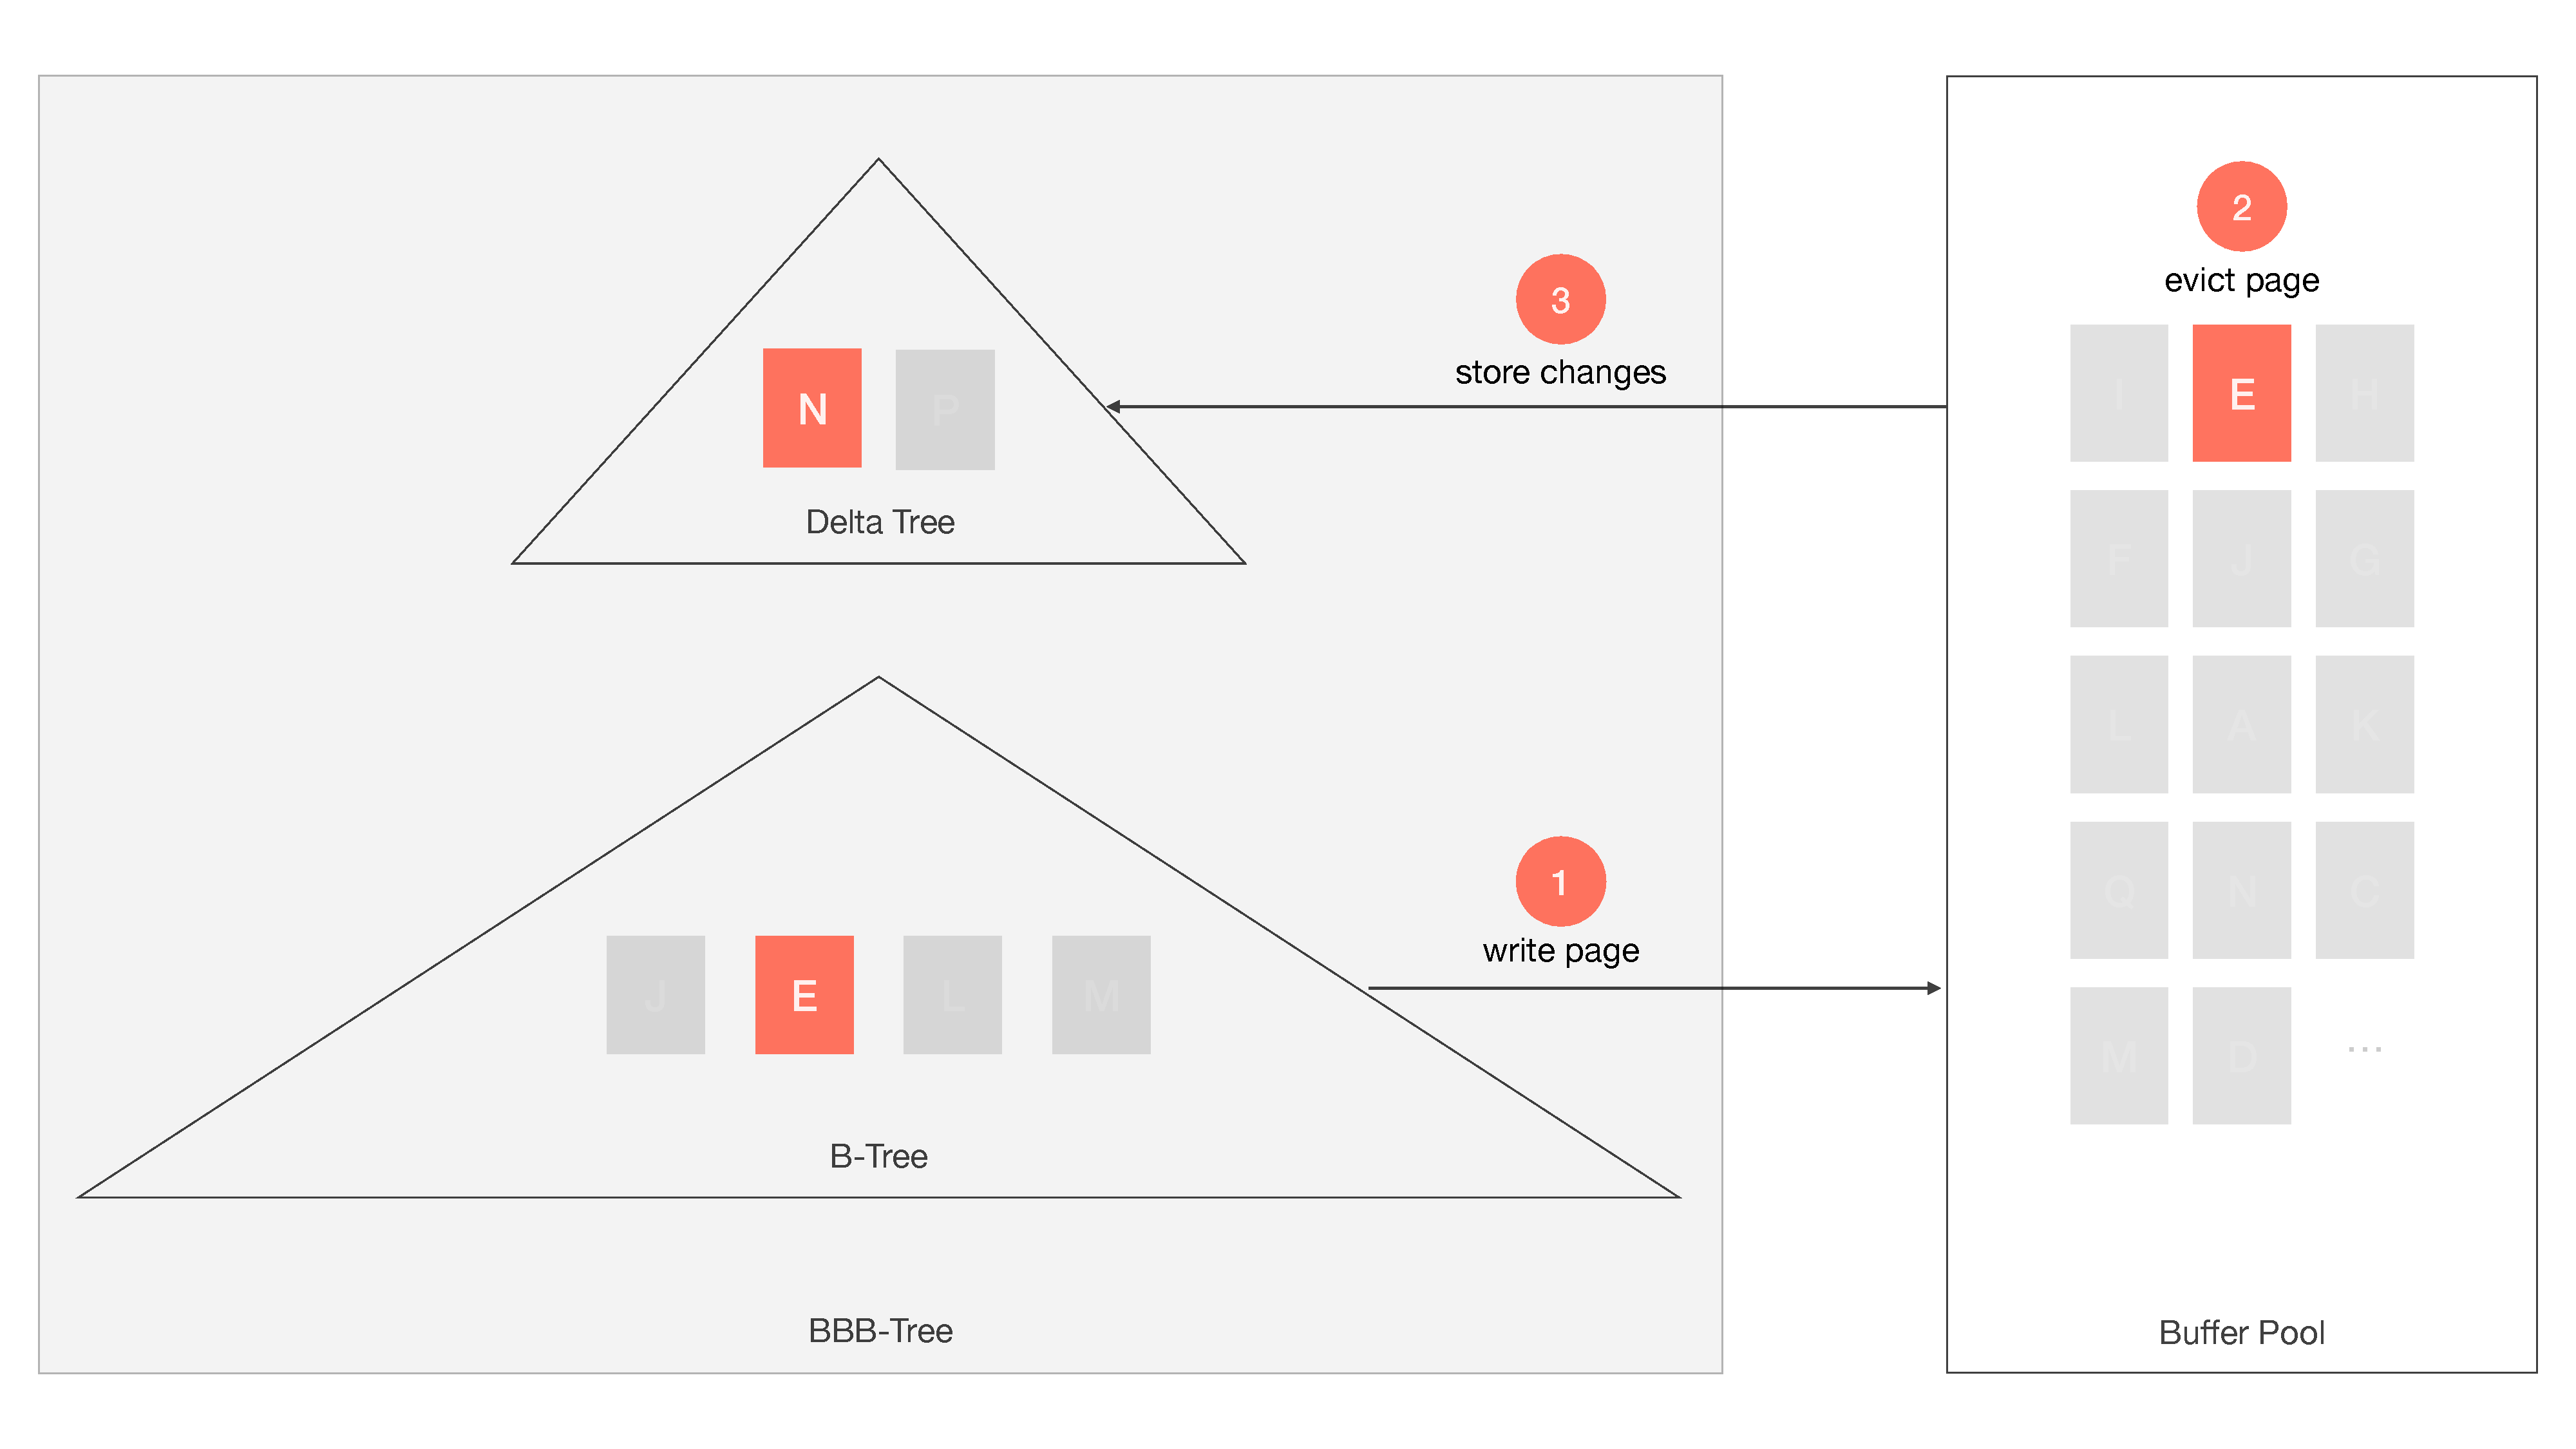
\includegraphics[width=0.99\textwidth]{figures/delta_tree.pdf}
  \caption{High-level architecture of the data structure. We add a Delta-Tree to a B-tree. When evicting a dirty page from the B-tree, we can buffer the changes of the B-tree pages instead of writing them to storage. When loading a page from storage, we apply all buffered changes to it before returning it to the B-tree.}
  \label{fig:delta-tree}
\end{figure}

We avoid writing a page to storage if changes are small.
To achieve this, we introduce a Delta Tree that acts as a hesitation layer, as illustrated in \autoref{fig:delta-tree}.
When evicting a dirty page, we can buffer the changes of the B-tree pages instead of writing them to storage immediately.
We can just discard the page, saving us the write to storage.
When loading a page from storage, we apply all buffered changes to it before returning it to the B-tree.
Only when enough changes accumulate, we write the full page to storage.

\inlinesection{Reduce Write Amplification.}
Write amplification in a B-tree happens at the point of evicting a page to storage.
The buffer manager is only aware that a page is dirty and needs to be written to storage.
It does not know which parts of the page changed.
Therefore, we keep track of the modifications made to each page in the B-tree.
Our component interacts with the buffer manager to intercept the eviction of dirty pages.
When evicting a dirty page, we can buffer the changes in the Delta Tree instead of writing them to storage immediately.
This way, we can defer small random writes until we have enough changes to justify a full rewrite to storage.
In the Delta Tree we can batch changes to the same page.

\inlinesection{Maintain Read Performance.}
To nodes in memory, this method is transparent.
When searching pages in memory, we do not incur overhead.

The only time we incur overhead is when loading a page from storage or unloading it to storage.
We argue that this overhead is acceptable, as we are already loading a page from storage.
The overhead of applying the buffered changes is small compared to the \ac{IO} operation.

However, the buffering layer itselt is a disk-based data structure, which migh require \ac{IO} operations to look up buffered changes.
We will be analyzing the overhead in \autoref{chap:evaluation}.    % TODO: Make sure that we do.
% i.e. there is an incentive to keep the delta tree small.
% TODO: Maybe we have more read amplifciation though because we also have IO to load the delta tree to apply changes.

\inlinesection{Maintain Concurrency.}
The Delta Tree is separate from the B-tree.
Therefore, we do not compromise concurrency of the B-tree itself, since we do not introduce further locking in the B-tree itself.
The Delta Tree can be implemented as a B-tree variant itself, allowing for high concurrency.

\inlinesection{Maintain Simplicity.}
The modifications we introduce to the B-tree itself are minimal.
Within the B-tree, we only need to track the modifications made to the nodes.
Essentially, we mark entries as dirty. 

The Delta Tree is a separate component that interacts with the buffer manager.
We do not dictate how the buffer manager is implemented or how it manages pages.
As a result, we maintain a low coupling between the data structure and the storage manager, allowing for optimizations in both layers independently.
For example, pointer swizzling is an optimization that could be applied with our method.

The Delta Tree itself is a B-tree variant, which we already have present in our system.
Therefore, we can reuse existing code and concepts, reducing implementation complexity.
Neither do we assume any special hardware features, making our approach broadly applicable across different storage media.

% Learned from related work that we want to turn small writes into large sequential writes by batching them.
% Obervation: Write amplification in B-trees is caused at the point of eviction. This is the point in time to buffer to defer a write.
% Uptain the happy path. We don't want any overhead for reads like a delta chain. At least not everytime we read from memory.

% Write out record-level updates on the page to another tree.
% A hesitation layer between B-tree and buffer manager.
% A buffer that can defer the write of a B-tree node. 
% When evicting a dirty page, we buffer the changes in memory instead of writing them to storage immediately.
% We can just discard the page, saving us the write to storage.
% To nodes in memory this is completely transparent. 
% Only when enough changes accumulate, we write the full page to storage. 
% When loading a page from storage, we apply all buffered changes to it before returning it to the B-tree.
% This way, we can turn many small random writes into few large sequential writes.
% We use a B-tree to buffer deltas. 

% Figure: Diagram of the architecture with the new layer.
\section{Data Structure Modifications}
% Figure: B-tree and 3B-tree (B-tree plus its Delta Tree, called by the Buffer Manager)
\subsection*{Buffer Manager}
The buffer manager is the component that decides when a page is evicted from memory and when a page is loaded into memory.
At the same time, the buffer manager should not be aware of any semantics of its pages.
More specifically, it does not know if it is evicting or loading pages of a B-tree or any other data structure.
However, we require specific logic to be executed when evicting or loading pages of a B-tree.
We need a way to inject this logic into the buffer manager without leaking B-tree specific logic into the buffer manager itself.
Therefore, users can register function pointers that are invoked at eviction time and loading time.
That way, the buffer manager remains agnostic of the semantics of its pages.

\subsection*{B-tree}
\begin{enumerate}
  \item \textbf{Tracking Write Amplification:}
We need to be aware of the degree of write amplification per node. 
Whenever we modify a node, for example through an insertion or a node split, we keep track of the amount of bytes that were changed.
Then, in relation to the page size, we can determine the write amplification of the node.
Based on that parameter, we can decide if a write operation to external storage is justified, or if we want to defer it.
  \item \textbf{Tracking Deltas:} 
We need to determine the changes that occurred on a node since the last time it has been loaded from external storage.
To that end, each entry on a node has an additional "state" field that indicates if the entry was inserted, updated, or deleted since the last time the node was loaded from external storage.
That way, we can buffer the "delta" image of a node at eviction-time and apply it again at loading time to ensure that we can reconstruct the logical state of a node when it is accessed again at a later point in time.
\item \textbf{Injecting Callbacks:}
As described above, we need to execute specific logic at eviction time and loading time of a B-tree page.
However, the B-tree has no control over the point in time a page is evicted or loaded.
Therefore, we inject callbacks into the buffer frames that are later invoked by the buffer manager.
Whenever we request a B-tree page from the buffer manager, we register function pointers for the Delta Tree.
At eviction- and loading-time, these function pointers are called by the buffer manager to execute the necessary logic.
\end{enumerate}

Alternatively, we could have immediately inserted changes into the Delta Tree whenever a change occured on a B-tree node.
This way, we would not need to track changes on the B-tree nodes themselves.
However, this would introduce significant overhead on every write operation to the B-tree.
Should a node be changed multiple times while it is in memory, we would need to update the Delta Tree multiple times as well.
In that case, we have many updates to a B-tree node and therefore want to perform the write to storage anyway.
We would have introduced the most overhead for situations without any benefit.
Therefore, we only interact with the Delta Tree at eviction- and loading-time of a B-tree page instead.
Only if we decide to buffer changes, we insert them into the Delta Tree.
This way, we keep the overhead for B-tree operations minimal.

\subsection*{Delta Tree}
The Delta Tree is the component that buffers changes of B-tree nodes.
The Delta Tree itself is a B-tree with \ac{PID}s as keys and lists of changes as values.
The buffer manager calls back the Delta Tree everytime a dirty B-tree page is evicted from memory or loaded into memory.

\begin{enumerate}
  \item \textbf{Eviction Time:}
The Delta Tree can decide if a B-tree page should be written to storage or not based on the write amplification of the page.
Should it decide to not write the page to storage, it buffers its changes.
It does so, by scanning the node for entries that were marked as dirty and inserting them into its own B-tree.
The buffer manager is informed that the page does not need to be written to storage anymore and can simply be discarded.

Should it decide to continue writing the page to storage, it simply returns and the buffer manager writes the page to storage as usual.
In this case, we clean the state of the B-tree page and remove any buffered changes from the Delta Tree, as it is now in sync with storage.

  \item \textbf{Loading Time:}
When loading a B-tree page from storage, the Delta Tree looks up if there are any buffered changes for that page.
If so, it applies the changes to the page before returning it to the B-tree.
Together with the state of the page on storage, we can reconstruct the state of the page in memory.

When changes were applied, we keep them in the Delta Tree, as they might be useful for future evictions.
This way, we perform less updates to the Delta Tree and can keep the state of the B-tree page clean.
Should there be no further changes to that page, the next eviction can simply discard the page without any writes.
\end{enumerate}

The Delta Tree itself contains pages that are managed by the buffer manager.
Its pages can be evicted to storage as well.
Therefore, we want to keep the Delta Tree small to batch changes more effectively.

\section{Implications on Write Amplification}
We can illustrate the effect of our approach on write amplification with a simple example.
\autoref{fig:delta-tree-example} shows a B-tree with updates across three nodes with \ac{PID}s {1, 2, 4}.
In a traditional B-tree, we would need to write all three pages to storage.
Assuming a page size of 4 KB and each update being 64 B, the write amplification is $(4096 B / 64 B) * 3 = 192$.

With our approach, we can buffer the changes of the three pages in the Delta Tree.
In this example, the Delta Tree only needs to write one page to storage, containing the three updates.
Assuming a page size of 4 KB again and approximating the delta entries to be 64 B each, the write amplification is now $4096 B / (3 * 64 B) = 21.33$.
In this simple example, we have reduced the write amplification by a factor of >9.

This demonstrates the goal of our approach: batching small writes on many distinct pages into larger writes on fewer pages.
This way, we can reduce the number of pages written to storage for a given set of updates, thereby reducing write amplification.

\begin{figure}[htpb]
  \centering
  \begin{subfigure}[t]{0.95\textwidth}
    \centering
    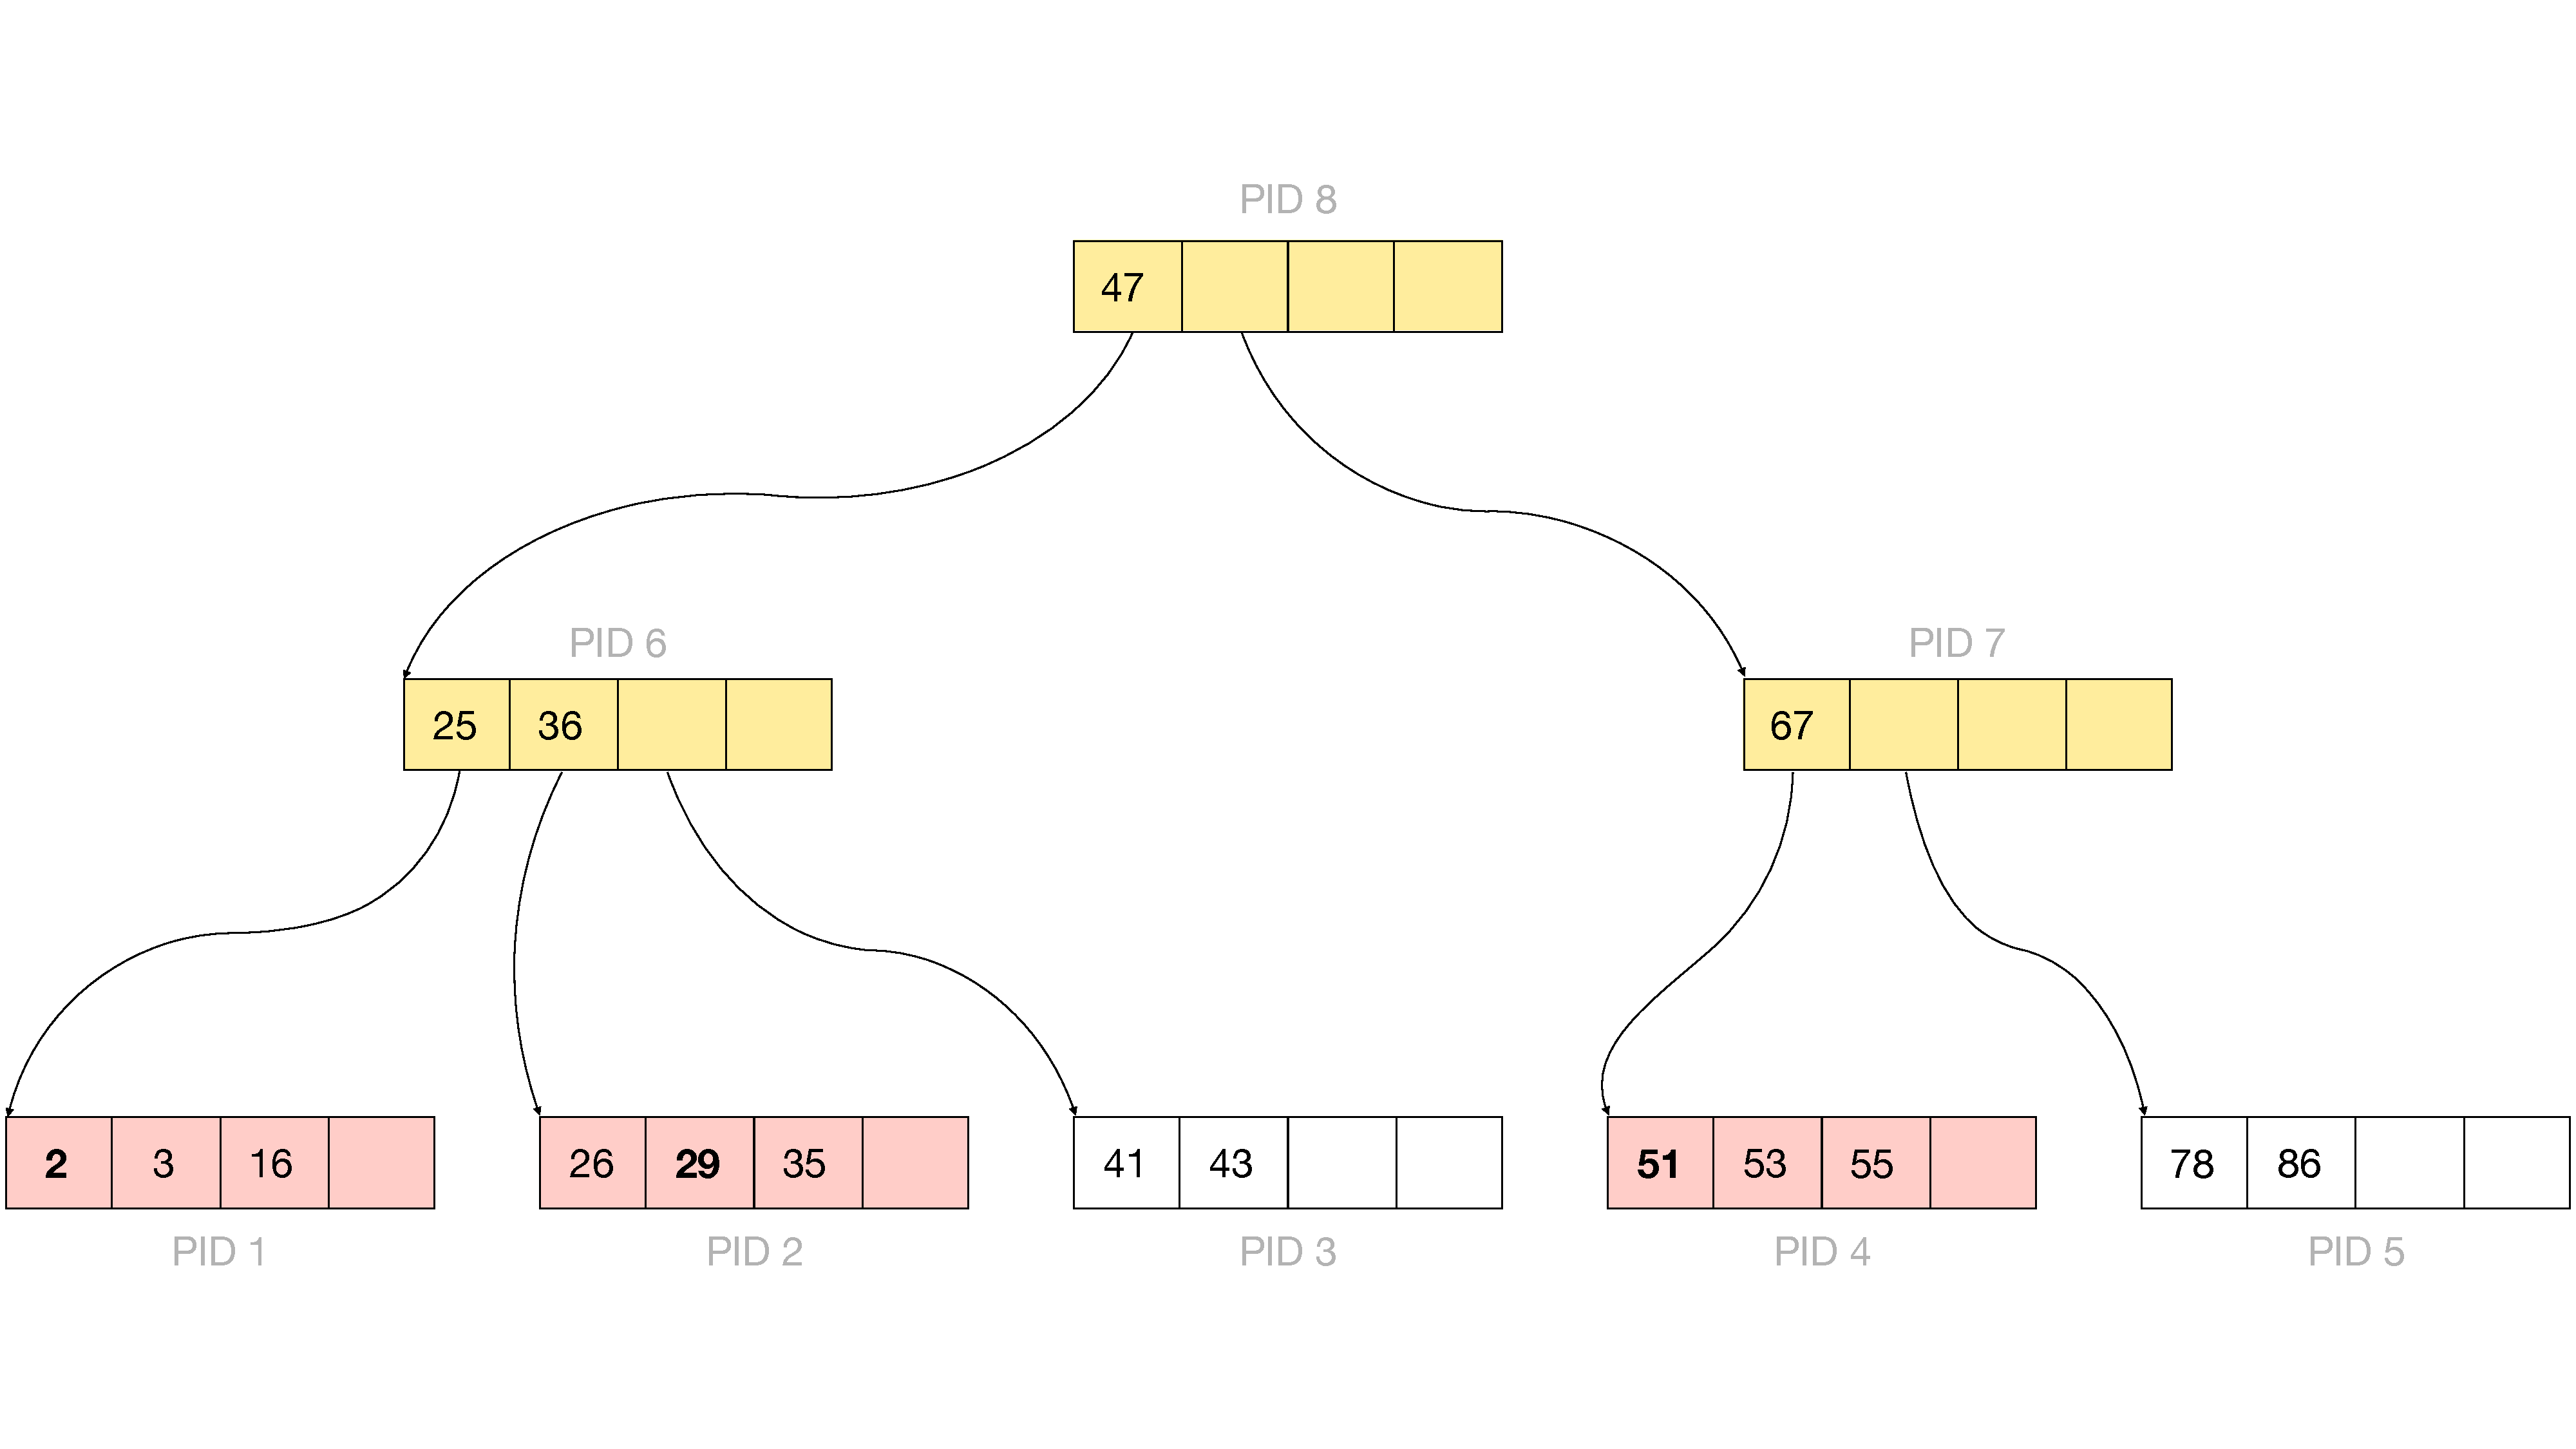
\includegraphics[width=\textwidth]{figures/b_tree_with_pid.pdf}
    \caption{A B-tree with updates to nodes with \ac{PID} {1, 2, 4}.}
  \end{subfigure}
  \hfill
  \begin{subfigure}[t]{0.95\textwidth}
    \centering
    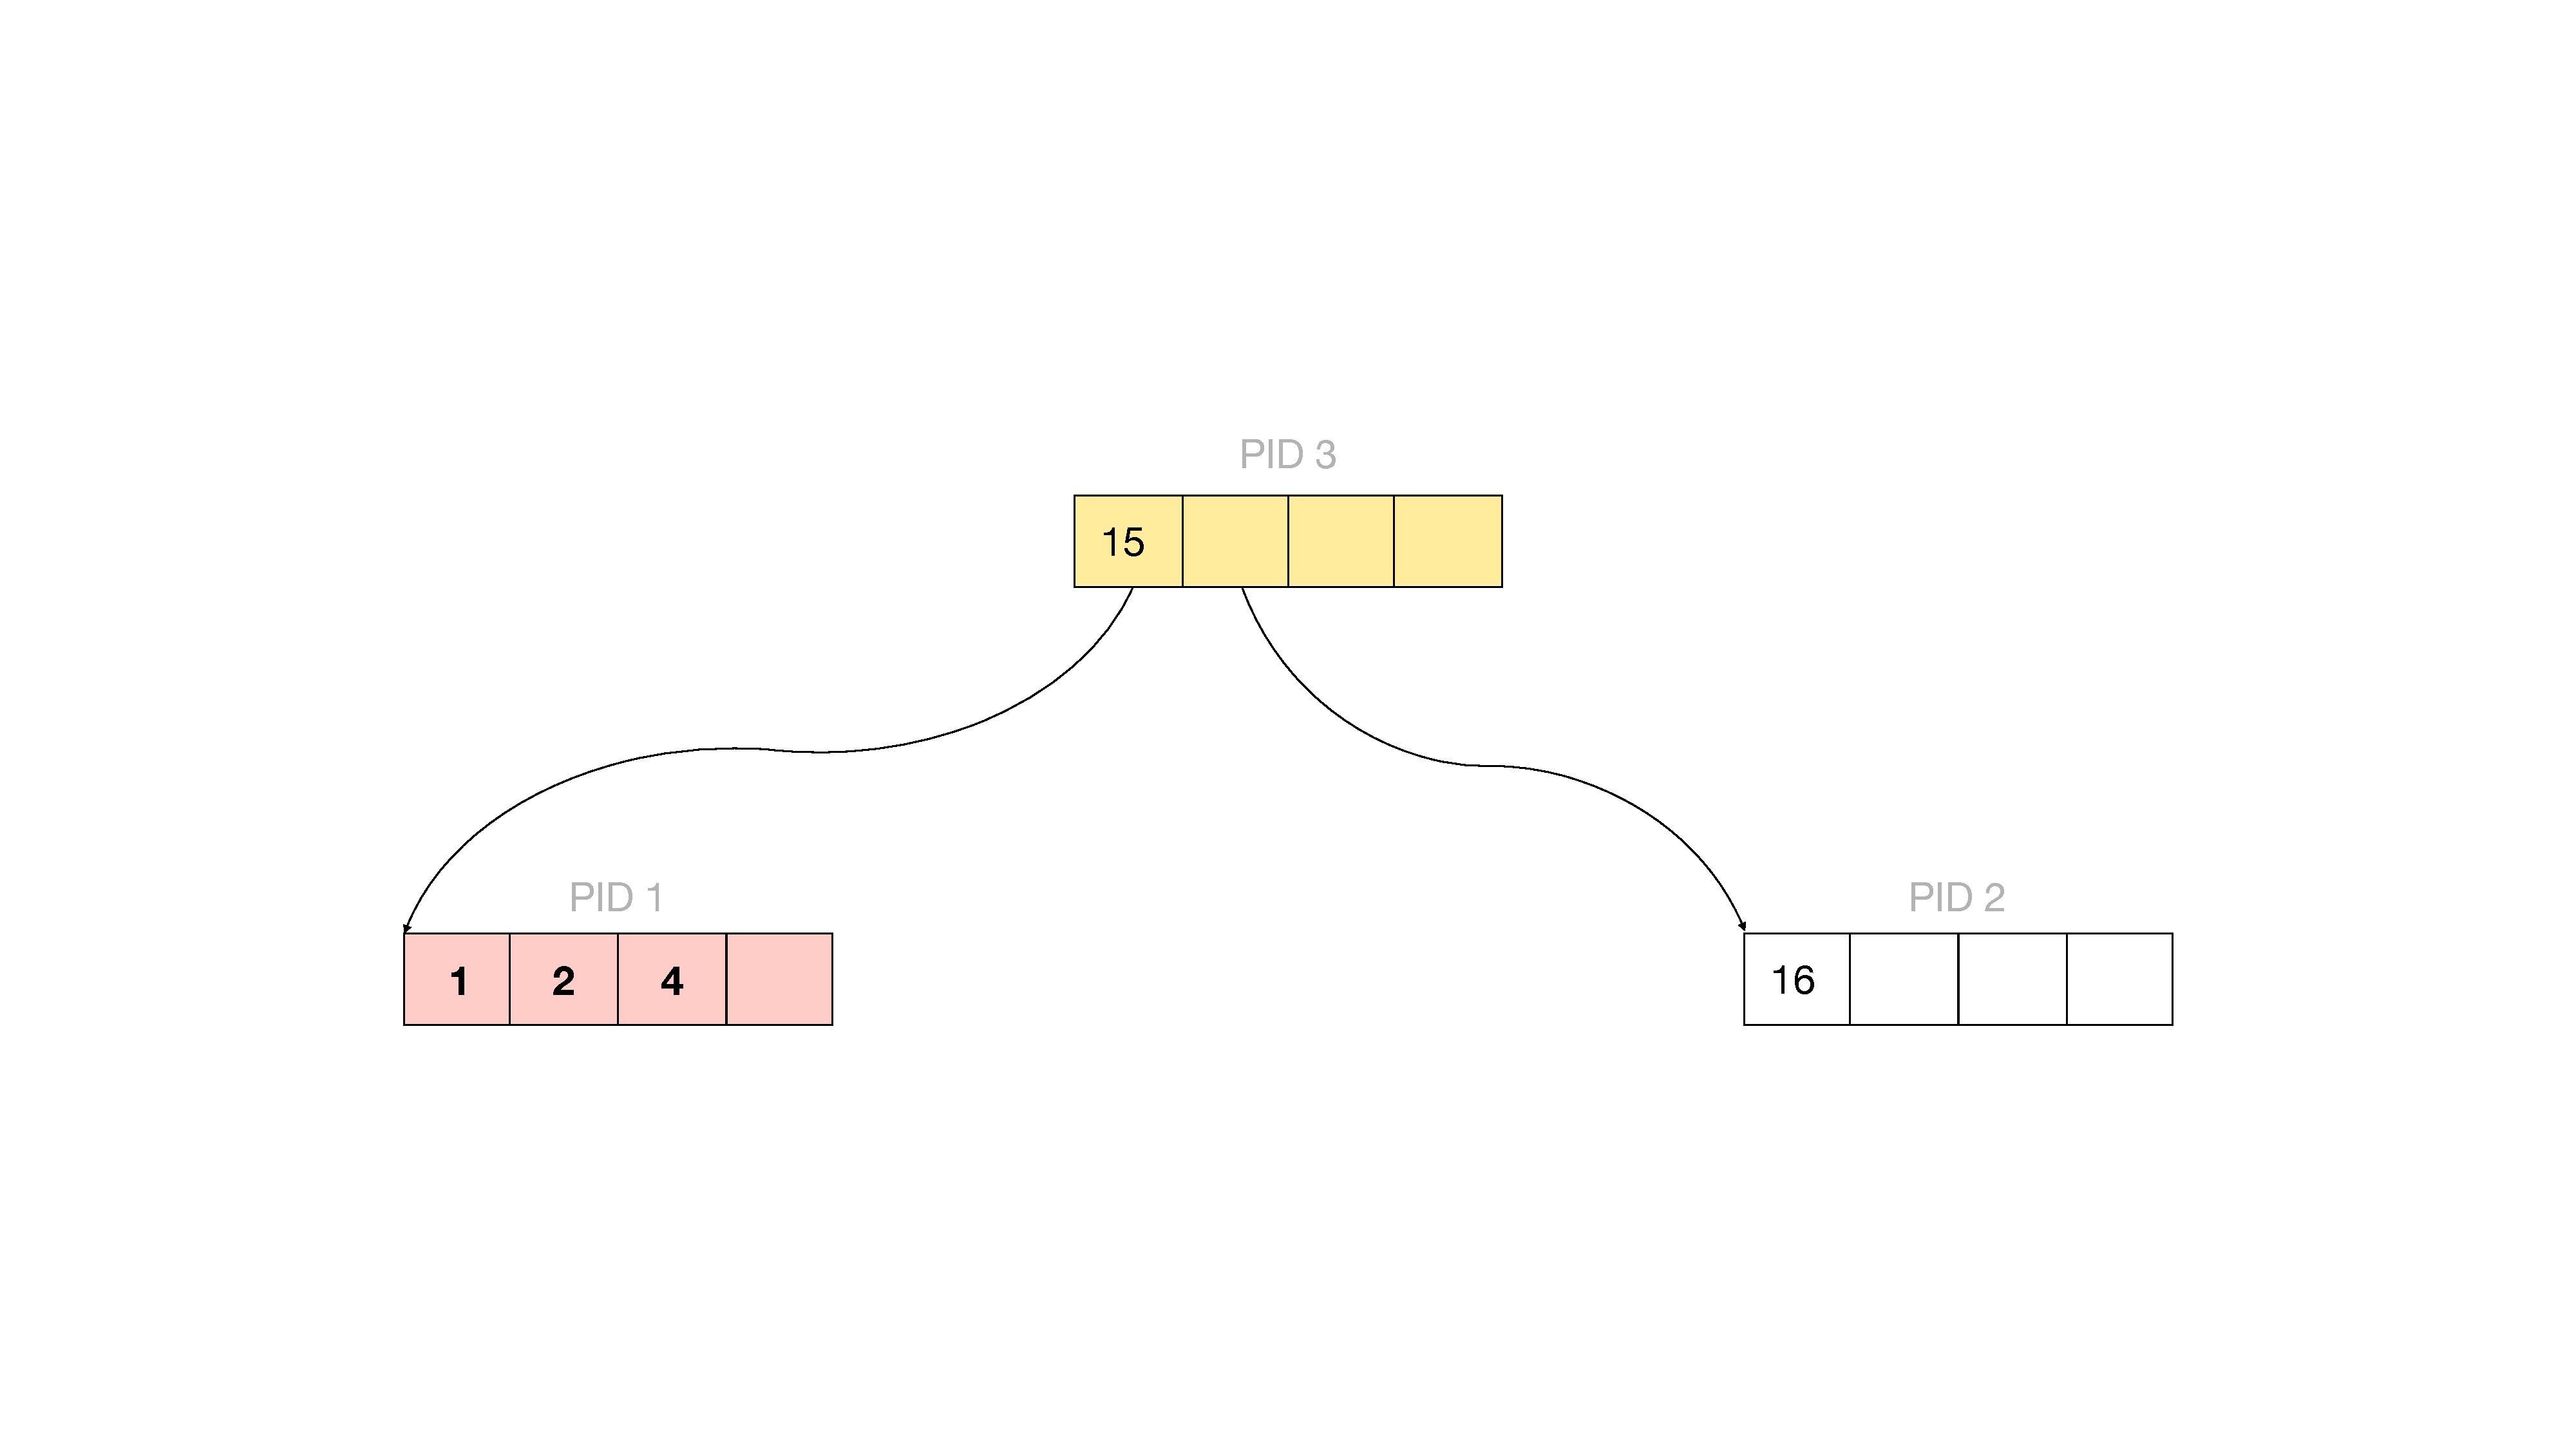
\includegraphics[width=\textwidth]{figures/delta_tree_update.pdf}
    \caption{The corresponding Delta Tree. Buffered the changes of B-tree nodes by their \ac{PID}s {1, 2, 4}.}
  \end{subfigure}
  \caption{Example of a B-tree and its corresponding Delta Tree. The B-tree has three updated nodes marked in red. In this example, we require only one page write for the Delta Tree instead of three writes for the B-tree.}
  \label{fig:delta-tree-example}
\end{figure}

\chapter{Implementation}

% \section{Environment and Tools Used}

\section{System Architecture}
% TODO: Figure from System Architecture

% We have implemented our system according to \autoref{fig:db-architecture} in C++. 
In the following, we inspect our particular implementation for each component.

% Slotted Page Nodes to address variable size keys/values
% Keys in index can be variable, Values are TID
% Key in Delta-Tree is PageID to fixed-size, Values are variable-size because deltas for a particular page can be of any size.

\subsection*{Buffer Manager}
% Our buffer manager serves our system with pages, transparently swapping them between memory and external storage.
% Upon construction, it receives a page_size that determines the fixed-sized number of bytes of every page in the system, as well as a page_count that determines the number of pages that can be present in the memory pool at once.

% fix_page
% unfix_page

% Serves pages between memory and storage
% Buffer Frames get a function pointer from an `PageLogic` interface that returns a bool whether the page should be written out or not.

\subsection*{Slotted Pages}
% TODO: Figure of Slotted Pages

% Support for variable sized values

\subsection*{B-Tree}
% Templated B-Tree on Key/Value Type
% Support for variable sized keys/values
% TODO: Maybe explain my B-Tree node structure for leafs and inner nodes like marcus müller does in his paper.
% Then its easiert to show the changes that we make through tracking.

\subsection*{BBB-Tree}
% Templates on PID and Deltas
% Contains a B-Tree and a Delta Tree
% Templated on Key/Value type.

\subsection*{Database}

\section{Algorithms for Lookups, Insertion, Deletion, and Rebalancing}

% Approximating the write amplifciation: e.g. an split and following insert can lead to more than the node size to change.
% Explain how we track state on a page and ensure that we do not loose changes. Delta Image + Storage Image = Current Image.
% Go into tracking Write Amplification and Tracking Changes for each.
% Approximating the write amplifciation: e.g. an split and following insert can lead to more than the node size to change.
\subsection*{Lookup}

\subsection*{Insertion}

\subsection*{Deletion}

\subsection*{Rebalancing}

\section{Testing and Verification}
% Unit Tests

\section{Challenges and Trade-offs}
% Want to keep compactification. Otherwise we could put changes in delta tree and then do unneccessary splits because the node does not have enough space after applying the changes again witout compactification.

% After a node split we generally want to write out the page because it carries a lot of information and compactification work savings.
% Problem of recursive calls to the Delta Tree. Locking the tree when operating on it. Otherwise it could access uninitialized nodes during splits for example.

% Scanning Deltas when evicting VS. keeping the DeltaTree up to date during manipulation of the B-Tree.

% Want to keep Deltas in the tree after applying them to be able to just throw them away when only reading. Less changes to the tree
% However: what do we do with stale deltas? Do we want to apply the at some point?
% We have an incentive to keep the Delta Tree small to batch changes more effectively. Therefore we can evict changes from the Delta Tree if they have not been used for a while.
% Also we should only track small changes. If a page has a lot of changes, it is better to write it out and not track it anymore.


\chapter{Evaluation}
\label{chap:evaluation}
% "Moreover, under large record size (e.g., 1KB and above), B+ tree tend to have smaller write amplification than LSM-tree." - from "Closing the B+-Tree vs. LSM-Tree Write Amplification Gap on Modern Storage Hardware with Built-in Transparent Compression", Qiao et al., FAST 2022
% Good evaluation paper: https://dl.acm.org/doi/pdf/10.1145/3183713.3196895
% To adhere to the DAM model, can't we assume that all inner nodes are cached in memory, but leafs are not? see "A Comparison of Fractal Trees to Log-Structured Merge (LSM) Trees"

% Question 0: How much write amplification do we have in a traditional B-tree. How much in our approach? Show the bytes inserted by the user, the bytes written to the tree, the bytes written to storage.
% Question 1: Does the approach reduce write amplification compared to a traditional B-Tree?
% Question 2: How does the approach affect read and write performance compared to a traditional B-Tree and LSM-Tree?
% Question 3: How does the approach affect latency/throughput?
% Question 4: How does the approach affect space utilization?
% Question 5: How does the approach affect memory usage and CPU utilization?
% Question 6: How does the approach scale with different types of workloads (read-heavy, write-heavy, mixed)?
% Question 7: How does the approach perform with different types of page sizes and delta sizes?

% Observations:
% We write a lot in the Delta Tree, to delete entries. Less fanout if we dont compactify often enough.

\section{Experimental Setup}
% Hardware specs
% Dataset, distribution
% Workloads (insert-heavy, read-heavy, mixed)
% Baselines (B-Tree, LSM-Tree)
% Metrics (write amplification, throughput (ops/s), latency, space utilization, memory usage, CPU utilization)

\section{Results and Analysis}
\subsection{Write Amplification}

\begin{figure}[htbp]
  \centering
  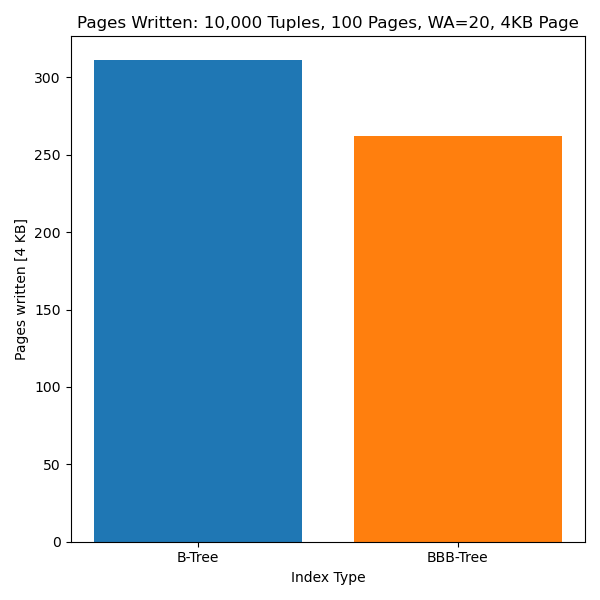
\includegraphics[width=0.6\textwidth]{figures/evaluation/10K_tuples_20_wa.png}
  \caption{Comparison of B-Tree and BBBTree performance for 10,000 insertions, building the index from scratch. We observe 15\% reduction in write amplification with our approach.}
  \label{fig:btree-vs-bbbtree-10000}
\end{figure}


\begin{figure}[htbp]
  \centering
  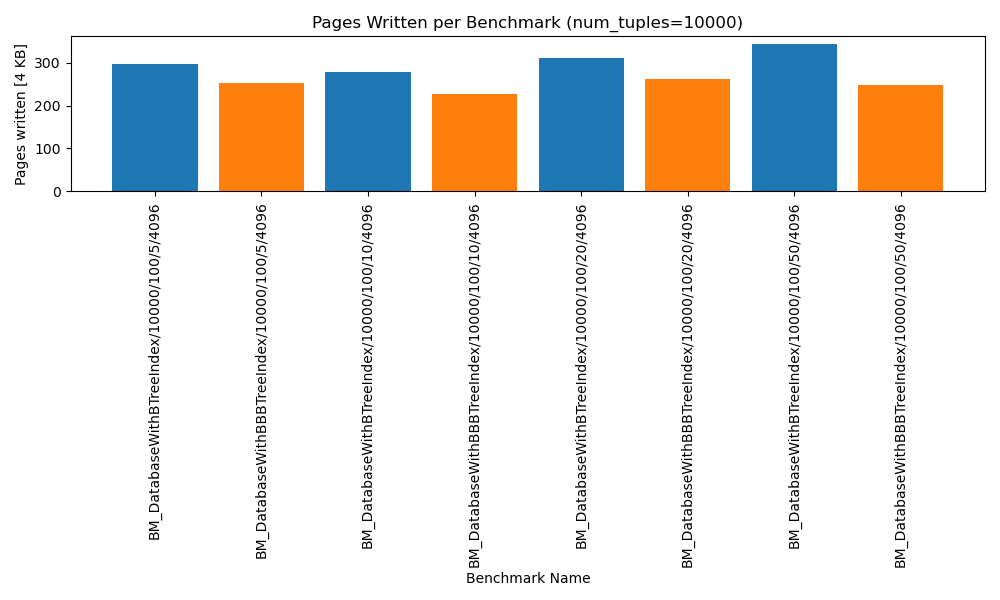
\includegraphics[width=0.8\textwidth]{figures/evaluation/10K_tuples_all_wa.png}
  \caption{Comparison of B-Tree and BBBTree performance for 10,000 insertions, building the index from scratch. We observe reduction in write amplification across different write amplification thresholds.}
  \label{fig:btree-vs-bbbtree-10000-all-wa}
\end{figure}

\begin{figure}[htbp]
  \centering
  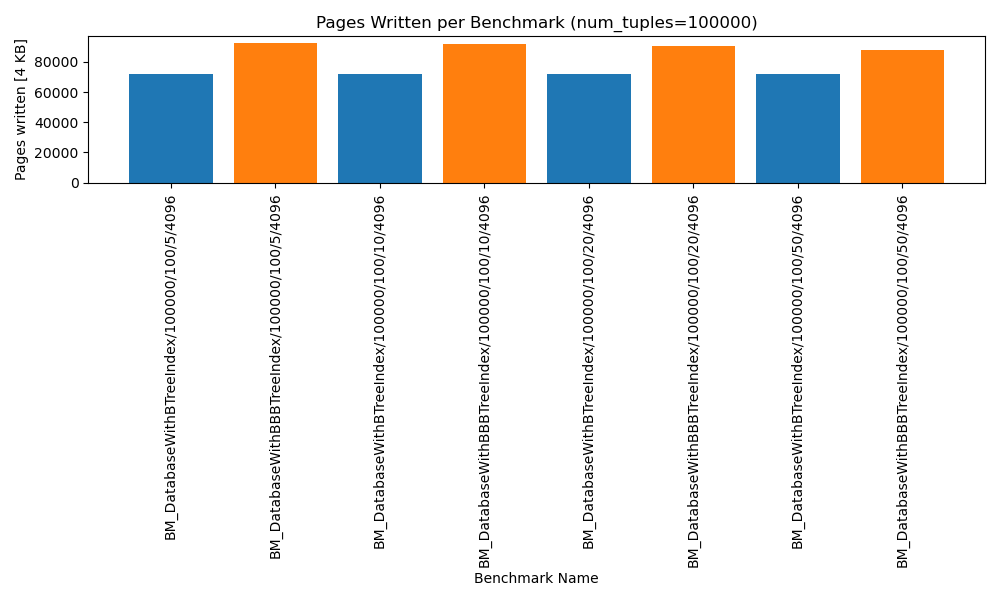
\includegraphics[width=0.8\textwidth]{figures/evaluation/100K_tuples_all_wa.png}
  \caption{Comparison of B-Tree and BBBTree performance for 100,000 insertions, building the index from scratch. We observe increase in write amplification across different write amplification thresholds.}
  \label{fig:btree-vs-bbbtree-100000-all-wa}
\end{figure}

% Write Amplification vs. Data size
% Write Amplification vs. Workload type (read-heavy, write-heavy, mixed)
% Number of writes to storage vs. workload type
% Average IO operations per update (baseline vs. our approach)

\subsection{Latency and Throughput}
% Latency vs. Workload type
% Throughput vs. Workload type
% Latency vs. Data size
% Throughput vs. Data size

\subsection{Space Utilization and Memory Overhead}
% Space Utilization vs. Data size (probably need more pages for fewer entries because slot size increases with delta tracking)
% 

\subsection{Sensitivity Analysis}
% WA vs Key Size
% WA vs Page Size
% WA vs Buffer Size
% WA vs Delta Size

\section{Discussion}
% “Our approach reduces write amplification by 40–60% while maintaining within 5% of baseline read latency.”
\chapter{Discussion and Future Work}
\section{Summary of Findings}
\section{Limitations}
\section{Future Directions}
% Other data strcutured than B-Tree that have more batching effect
% Use levelling that keeps inserting into another level if write amplification is too high. Better batching.
% When the Delta Tree gets too big, we just transfer random writes from one tree to another.
% Therefore it only makes sense to track small changes. If a page has a lot of changes, it is better to write it out and not track it anymore.
\section{Potential Applications}

\chapter{Conclusion}
\section{Recap of Contributions}
\section{Final Thoughts}
% TODO: add more chapters here

\appendix{}
\chapter{Appendices}
\section{Pseudocode}
\section{Additional Graphs and Tables}
\section{Configuration Files / Benchmarking Scripts}

\microtypesetup{protrusion=false}

\addchap{Abbreviations}
\begin{acronym}
	\itemsep-.25\baselineskip
	\acro{TUM}[TUM]{Technical University of Munich}
	\acro{WA}[WA]{Write Amplification}
	\acro{LSMT}[LSM-Trees]{Log-Structured-Merge-Trees}
	\acro{SSD}[SSDs]{Solid State Drives}
	\acro{DBMS}[DBMS]{Database Management Systems}
	\acro{CPU}[CPU]{Central Processing Unit}
	\acro{DRAM}[DRAM]{Dynamic Random Access Memory}
	\acro{IO}[I/O]{Input/Output}
	\acro{TID}[TID]{Tuple ID}
	\acro{CAS}[CAS]{Compare-And-Swap}
	\acro{WAL}[WAL]{Write-Ahead Log}
	\acro{DAM}[DAM]{Disk-Access-Model}
	% TODO: add acronyms
\end{acronym}

\listoffigures{}
\listoftables{}
\microtypesetup{protrusion=true}
\printbibliography{}

\end{document}
